\documentclass[a4paper,11pt,oneside]{article}
\renewcommand*{\baselinestretch}{1.04}
\usepackage[margin=2.5cm]{geometry}

\usepackage[T1]{fontenc}
\usepackage[utf8]{inputenc}
\usepackage{lmodern}

\usepackage{paralist}
\pltopsep=0pt
\plitemsep=0pt
\plparsep=0pt

\def\+{+}

\makeatletter
\catcode`\ =12\let\@nl@space= \catcode`\ =10
\newcount\@nl@rlevel
\newcount\@nl@llevel
\@nl@llevel=-1

\def\@nl{%
  \catcode`\ =12
  \global\@nl@rlevel=0
  \futurelet\@nl@store\@nl@%
}
\def\@nl@gobble#1{\futurelet\@nl@store\@nl@}
\def\@nl@enditemize{
  \ifnum\the\@nl@rlevel<\the\@nl@llevel%
    \end{compactitem}%
    \egroup%
    \expandafter\@nl@enditemize%
  \else%
    \ifnum\the\@nl@rlevel=\the\@nl@llevel\else%
       \errmessage{Error: inconsistent identation}
    \fi%
  \fi%
}
\def\@nl@{%
  \ifx\@nl@store\@nl@space%
    \global\advance\@nl@rlevel by 1
    \expandafter\@nl@gobble%
  \else%
    \catcode`\ =10
    \ifx\@nl@store+%
      \ifnum\the\@nl@rlevel>\the\@nl@llevel%
        \bgroup%
        \@nl@llevel=\the\@nl@rlevel
        \begin{compactitem}%
      \fi%
      \@nl@enditemize%
      \item \expandafter\expandafter\expandafter\@gobble%
    \else%
      \ifx\@nl@store\@nl%
        \global\@nl@rlevel=-1\relax\@nl@enditemize\par
      \else\space\fi%
    \fi%
  \fi%
}
\makeatother

\def\magyarOptions{defaults=prettiest}
\usepackage[magyar]{babel}

\usepackage{amsmath,wasysym,mathtools,mleftright,relsize,amssymb}

\usepackage[stretch=10]{microtype}

\usepackage{xspace,mdframed,array}

\newmdenv{tetelframe}
\setcounter{secnumdepth}{-1}
\newcounter{tetel}
\newcommand{\tetel}[1]{\begin{tetelframe}\noindent\refstepcounter{tetel}\textbf{\thetetel.}~#1\end{tetelframe}}

\newcommand*{\ra}{\ensuremath{\rightarrow}\xspace}
\newcommand*{\RA}{\ensuremath{\Longrightarrow}\xspace}
\newcommand*{\LA}{\ensuremath{\Longleftarrow}\xspace}
\newcommand*{\app}{\ensuremath{\approx}\xspace}
\newcommand*{\lra}{\ensuremath{\leftrightarrow}\xspace}
\newcommand*{\LRA}{\ensuremath{\Longleftrightarrow}\xspace}

\newcounter{theorem}[tetel]
\renewcommand*{\thetheorem}{\thetetel.\arabic{theorem}}
\newcommand*{\theoremlike}[1]{\refstepcounter{theorem}{\textbf{\thetheorem.~#1:}}\xspace}
\newcommand*{\thm}{\theoremlike{tétel}}
\newcommand*{\example}{\theoremlike{példa}}
\newcommand*{\prob}{\theoremlike{probléma}}
\newcommand*{\alg}{\theoremlike{algoritmus}}
\newcommand*{\dfn}{\theoremlike{definíció}}
\newcommand*{\lemma}{\theoremlike{lemma}}
\newcommand*{\corr}{\theoremlike{következmény}}
\newcommand*{\proof}{\textit{bizonyítás:}\xspace}
\newcommand*{\noproof}{\textit{nem bizonyítjuk}}
\newcommand*{\qed}{\hfill\ensuremath{\square}}
\newcommand*{\RR}{\mathbb{R}}
\newcommand*{\ZZ}{\mathbb{Z}}
\newcommand*{\Nat}{\mathbb{N}}
\newcommand*{\GF}{\textrm{GF}_2}
\newcommand*{\MM}{\mathcal{M}}
\newcommand*{\NN}{\mathcal{N}}
\newcommand*{\UU}{\mathcal{U}}
\newcommand*{\FF}{\mathcal{F}}
\newcommand*{\BB}{\mathcal{B}}
\newcommand*{\CC}{\mathcal{C}}
\newcommand*{\T}{\mathrm{T}}
\newcommand*{\IP}{\textit{IP}}
\newcommand*{\LP}{\textit{LP}}
\newcommand*{\DLP}{\textit{DLP}}
\newcommand*{\DIP}{\textit{DIP}}

\newcommand*{\DataIn}{\textsc{Input}:\xspace}
\newcommand*{\DataOut}{\textsc{Output}:\xspace}

\newcommand{\vertle}{\rotatebox{90}{$\mkern-2mu\le$}}
\newcommand{\vertgt}{\rotatebox{90}{$\mkern-2mu>$}}
\DeclareMathOperator*{\argmax}{arg\,max}

\usepackage{tikz}
\usetikzlibrary{positioning,calc,shapes.geometric,through}
\let\tikzpictureunpatched\tikzpicture
\def\tikzpicture{\catcode`\^^M=5\tikzpictureunpatched}
\tikzset{
  vertex/.style={shape=circle,fill=black,inner sep=0pt,
    font=\nullfont,minimum width=4pt}
}

\title{Rendszeroptimalizálás vizsgatételek (2015/2016.~második
  félév)}
\author{Marussy Kristóf}

%\makeatletter
%\usepackage[pdftitle={\@title},pdfauthor={\@author}]{hyperref}
%\makeatother

\begin{document}

\makeatletter
\catcode`\^^M=\active%
\let^^M=\@nl%
\makeatother

\maketitle
\thispagestyle{empty}

\begin{ocg}[printocg=never]{ForkMe}{1}{1}
  \begin{tikzpicture}[remember picture, overlay]
    \node[rotate=-45, shift={(0, -3.2cm)}] at (current page.north east) {%
      \begin{tikzpicture}[remember picture, overlay]
        \node at (0pt, 0pt) {\pgfuseshading{forkmeshading}};
        \node[text=forkmefg] at (0pt, 0pt) {%
          \large\bfseries\clear Fork me on GitHub};
        \draw[forkmefg!70!forkmebg, dashed, line width=.08em, dash pattern=on .5em off 1.5\pgflinewidth] (-600pt,12pt) rectangle (600pt,-12pt);
      \end{tikzpicture}%
    };
    \node [anchor=north east] at (current page.north east) {
      \href{https://github.com/kris7t/ropi}{\parbox[t][5cm]{5cm}{\hfill}}};
  \end{tikzpicture}
\end{ocg}


\section{Lineáris programozás}

\tetel{Az optimális hozzárendelés problémája, Egerváry algoritmusa.}

+ \example egy cég számos megrendelést kap különboző ``egyszemélyes'',
  egyforma idő alatt elvégezhető munkák elvégzésére
  + kimutatást készítünk arról, hogy melyik dolgozó melyik munkát
    tudja elvégezni
  + cél a profit maximalizálása (lehető legtöbb munka elvégzése)
+ \alg ``magyar módszer''
  + \DataIn $G = (F, L; E)$ páros gráf
  + \DataOut $M \subseteq G$ egy maximális méretű párosítás
  + induljunk ki egy tetszőleges (pl.~az üres) $M$ párosításból
  + \emph{alternáló út} = párosítatlan $F$-beli csúcsból indul, $\forall$
    második éle az $M$-hez tartozik
    + \emph{javító út} = olyan alternáló út, ami párosítatlan $L$-beli
      pontban ér véget
  + amíg találunk $J$ javítóutat (pl.~szélességi kereséssel) \RA $M
    \gets M - (J \cap M) \cup (J - M)$
+ \thm \label{thm:linprog:egervary:magyar}a ``magyar módszer'' valóban maximális párosítást talál
  $G$-ben
  + \proof $M \coloneqq \text{a párosítás, amit az algoritmus
    megtalált}$
  \begin{align*}
    F_1 &\coloneqq F - M, \text{az $M$ által le nem fedett $F$-beli
          pontok halmaza,}\\
    L_2 &\coloneqq \text{az $F_1$-ből alternáló úton elérhető pontok
          halmaza,} \\
    F_2 &\coloneqq \text{az $L_2$-beli pontok $M$ szerinti párjai,} \\
    L_3 &\coloneqq \text{az $F_1$-ből alternáló úton nem elérhető
          $L$-beli pontok halmaza,} \\
    F_3 &\coloneqq \text{az $L_3$-beli pontok $M$ szerinti párjai,} \\
    L_1 &\coloneqq L - M, \text{az $M$ által le nem fedett $L$-beli pontok
          halmaza}
  \end{align*}
  + vegyük észre, hogy $G$-ben nem vezethet $F_1 \cup F_2$ és $L_1
    \cup L_3$ között él
    \par
    {\centering\begin{tabular}{c|p{6cm}|p{6cm}}
      & \multicolumn{1}{c|}{$F_1$} & \multicolumn{1}{c}{$F_2$} \\\hline
      $L_1$ & $1$ hosszú javító út lenne & $\ge 3$ hosszú javító út lenne \\\hline
      $L_3$ & az $L_3$-beli csúcs $1$ hosszú alternáló úton elérhető lenne, azaz $L_2$-beli
            & az $L_3$-beli csúcs $\ge 3$ hosszú alternáló úton elérhető lenne, azaz $L_2$-beli
    \end{tabular}\par}
  + $F_1 \cup F_2$ $\forall$ szomszédja $L_2$-beli, $L_2 \cup F_3$ egy lefogó ponthalmaz
  + mivel épp $\lvert M \rvert = \lvert L_2 \cup F_3 \rvert$, $M$
    valóban maximális méretű \qed
+ \prob optimális hozzárendelés
  + \DataIn $G = (F, L; E)$ páros gráf, $w\colon E \to \RR$
    súlyfüggvény
  + \DataOut $M \subseteq G$ párosítás úgy, hogy $\sum_{e \in M} w(e)$
    maximális
  + az optimális hozzárendelés megoldható maximális súlyú
    \emph{teljes} párosítás keresésével
    + ha $\lvert F \rvert \ne \lvert L \rvert$, adjunk $G$-hez annyi
      csúcsot, hogy egyenlőek legyenek
    + legyen $G' = (F, L; E')$ teljes páros gráf ($E' = F
      \times L$), $w'(e) \coloneqq \text{\footnotesize$\begin{cases}
        w(e), &\text{ha $e \in E$,} \\
        0, & \text{ha $e \notin E$}
      \end{cases}$}$
    + $G'$ egy $M'$ maximális súlyú teljes párosítasa a $G$ maximális
      súlyú párosítása az $E' - E$ élek elhagyása után
    + $G$ maximális súlyú $M$ párosításához megfelelő $E' - E$ éleket
      hozzávéve $G'$ maximális súlyú teljes párosítását kapjuk
+ \dfn a $c\colon F \cup L \to \RR$ függvény \emph{címkézés} a $G =
  (F, L; E)$ páros gráfra és a $w\colon E \to \RR$ súlyfüggvényre
  nézve, ha $\forall e = \{ x, y \} \in E\colon c(x) + c(y) \ge w(e)$
+ \lemma a $w$ súlyfüggvénnyel súlyozott $G = (F, L; E)$ páros gráf
  tetszőleges $M$ teljes párosítására és tetszőleges $c$
  címkézésére igaz, hogy $\sum_{e \in M} w(e) \le \sum_{v \in F
    \cup L} c(v)$
  + \proof $\displaystyle \sum_{e \in M} w(e) \le \sum_{\mathclap{e = \{f, l\} \in M}}\, c(f) +
    c(l) \overset{\substack{\text{$\forall$ csúcs legfeljebb}\\\text{$1$-szer szerepel $M$-ben}}}{\le} \sum_{f \in F} c(f) + \sum_{l \in L} c(l) = \sum_{\mathclap{v \in F
    \cup L}}\, c(v)$ \qed
  + \dfn a $G$ gráf $e = \{x, y\}$ éle \emph{piros}, ha $c(x) +
    c(y) = w(e)$
  + \corr ha az $M$ teljes párosítás $\forall$ éle piros valamely $c$
    címkézésre nézve, akkor $M$ maximális súlyú teljes párosítás
+ \alg Egerváry algoritmusa
  + \DataIn $G = (F, L; E)$ páros gráf, $w\colon E \to \RR$
  súlyfüggvény
  + \DataOut $M \subseteq G$ \emph{teljes} párosítás úgy, hogy $\sum_{e \in M} w(e)$ maximális
  + 0.~lépés: legyen $M = \emptyset$, $c(v) = \begin{cases}
    \max_{y \in L, \{v, y\} \in E} w({v, y}), & \text{ha $v \in F$,} \\
    0, & \text{ha $v \in L$}
  \end{cases}$
  + 1.~lépés: a javító utas algoritmussal keressünk bővítsük $M$-et
    maximális élszámú párosítássá a piros részgráfban
    + ha $M$ most már teljes \RA STOP, $M$ a keresett párosítás, $c$ a
    keresett címkézés, $w(M) = c(M)$
  + 2.~lépés: $\delta \coloneqq \min \{ c(x) + c(y) - w(\{x, y\}) \mid
    \{x, y\} \in E, x \in F_1 \cup F_2, y \in L_1 \cup L_3 \}$
    + állítsuk elő a $c(v) \gets \text{\footnotesize$\begin{cases}
      c(v) - \delta, & \text{ha $v \in F_1 \cup F_2$,} \\
      c(v) + \delta, & \text{ha $v \in L_2$,} \\
      c(v), & \text{ha $v \in F_3 \cup L_1 \cup L_3$}
    \end{cases}$}$ új címkézést, majd GOTO 1.
+ \thm Egerváry algortimusa $O(n^2 e)$ lépésben maximális súlyú teljes
  párosítást állít elő
  + \proof a 0.~lépésben megadott $c$ valóban címkézés
  + a 2.~lépésben $\delta$ kiszámításához valóban van él $F_1 \cup
  F_2$ és $L_1 \cup L_3$ között
    + ha nem lenne, $N(F_1 \cup F_2) = L_2$
    + $\lvert F_1 \cup F_2 \rvert > \lvert F_2 \rvert = \lvert L_2
    \rvert$ miatt ekkor nem teljesül a Hall-feltétel \RA $\nexists$
    teljes párosítás!
  + a 2.~lépés után is címkézés marad $c$
    + csak az $F_1 \cup F_2$ és $L_1 \cup L_3$ között vezető élekre
    csökken $c(x) + c(y)$
    \par
    {\centering
      \begin{tabular}{c|c|c|c}
        & $F_1$ & $F_2$ & $F_3$ \\\hline
        $L_1$ & $-\delta$ (nem lehet piros) & $-\delta$ (nem lehet piros) & $0$ \\\hline
        $L_2$ & $-\delta + \delta$ & $-\delta + \delta$ & $+\delta$
                                                          (piros eltűnhet) \\\hline
        $L_3$ & $-\delta$ (nem lehet piros) & $-\delta$ (nem lehet piros) & $0$
      \end{tabular}\par}
    + $\delta$ definíciója garantálja, hogy továbbra is $c(x) + c(y)
      \ge w(\{x, y\})$
  + $M$ élei a 2.~lépés után is pirosak
    + csak $x \in F_3$, $y \in L_2$ élek színeződhetnek vissza (itt nőtt
      $c(x) + c(y)$)
    + ezek nem lehetnek $M$ élei, mert $F_3$ párja $L_3$, $L_2$ párja
    $F_2$
    + továbbra is van $F_1$-ből piros alternáló út $L_2$ csúcsaiba
  + egy iterációban vagy $M$, vagy $L_2$ elemszáma nő
   + $O(n)$ lépés után $M$ elemszáma mindenképp nő, mert ekkorra már $L_2$
     lefedné $L$-t
   + $O(n^2)$ iterációban $M$ maximális párosítás lesz
   + ezért $O(n^2 e)$ időben az algoritmus véget ér \qed

\tetel{A lineáris programozás alapfeladata, kétváltozós feladat
  grafikus megoldása. Lineáris egyenlőtlenségrendszer megoldása
  Fourier`--Motzkin eliminációval.}

+ legyen $A \in \RR^{m \times n}$, $x \in \RR^n$, $b \in \RR^m$, $c \in
  \RR^n$ \RA \emph{lineáris program}
+ \dfn \emph{linerási programozás alapfeladata}: $\min_{x} \{ cx : Ax
  \le b \}$
+ kétdimenziós feladat megoldása
  + az $p_1 x_1 + p_2 x_2 \ge k$ alakú feltétel $p_1 x_1 + p_2
  x_2 = k$ egyenese két félsíkra bontja a síkot
    + a $\ge$ jelnek megfelelő félsíkok metszete adja megengedett
      megoldások tartományát
  + ha $c = (q_1, q_2)$ \RA $q_1 x_1 + q_2 x_2 = 0$-val párhuzamos
  egyeneseket húzunk
    + minden egyenesre kiszámítjuk a célfüggvény értékét
    + a maximumhely a legnagyobb egyenes és a félsíkok metszetének
    közös pontja
  + általánosítás: \emph{hipersíkok} által határolt \emph{poliéder}
+ ekvivalens átalakítások
  + egyenlőtlenség megszorzása \emph{pozitív} számmal
  + két egyenlőtlenség összegének hozzávétele az egyenlőtlenségrendszerhez
  + \emph{nem} ekvivalens: szorzás negatív számmal
+ \alg Fourier`--Motzkin elimináció
  + $n$ változós lineáris program visszavezetése egy $n - 1$ változós
    $A^*$, $b^*$ lineáris programra
  + végül $1$ változós lineáris program megoldása
  + $(A|b)$ bővített együttható mátrix
    + szorozzuk pozitív számokkal a
      sorokat, hogy az $1$.~oszlopban csak $-1, 0, 1$ legyen
  + legyen $I$, $J$, $K$ rendre az $1$-gyel, $-1$-gyel és $0$-val
    kezdődő sorok indexeinek halmaza
  + $\RR^{\lvert K \rvert \times n} \ni (A_0|b_0) =$ $(A|b)$ $0$-val
    kezdődő sorai az első oszlop elhagyásával
  + $Ax \le b$ egy megoldása $x = (\lambda, \bar{x})$ alakú \RA $A_0
    \bar{x} \le b_0$ \RA mikor van megfelelő $\lambda$?
  + ha $J = \emptyset$ (nincs $-1$-gyel kezdődő sor)
    + $\forall i \in I : \lambda + \bar{a}_i \bar{x} \le b_j$ \RA
      $\lambda \le \min_{i \in I} b_i - \bar{a}_i \bar{x}$, ami mindig
      kielégíthető
    + $A^*, b^* =$ az $\bar{A}$-ból és $b$-ből az $i \in I$ indexű sorok
      elhagyásával kapott rendszer
  + ha $I = \emptyset$ (nincs $1$-gyel kezdődő sor)
    + $\forall j \in J : -\lambda + \bar{a}_j \bar{x} \le b_j$ \RA
      $\lambda \ge \max_{j \in J} \bar{a}_j \bar{x} - b_j$, ami mindig
      kielégíthető
    + $A^*, b^* =$ az $\bar{A}$-ból és $b$-ből az $j \in J$ indexű sorok
      elhagyásával kapott rendszer
  + ha $I \ne \emptyset$ és $J \ne \emptyset$ \RA
    $\forall i \in I : \lambda + \bar{a}_i \bar{x} \le b_j$ és
    $\forall j \in J : -\lambda + \bar{a}_j \bar{x} \le b_j$
    + $\forall i \in I, j \in J: \bar{a}_j \bar{x} - b_j \le \lambda
      \le \bar{b}_i - \bar{a}_i \bar{x}$ \RA $\forall i \in I, j \in J:
      (\bar{a}_i + \bar{a}_j) \bar{x} \le b_i + b_j$
    + $A^*, b^* =$ az $\bar{A}$ és $b$-ből $i \in I$ és $j \in J$
      indexű sorait az összes lehetséges módon összeadjuk, a $k \in K$
      indexű sorokat hozzávesszük és a csupa $0$ első oszlopot
      elhagyjuk
  + egyváltozós rendszer megoldása
    + ha $\exists k \in K : b_k < 0$ \RA a rendszer nem megoldható
    + ha $\max_{j \in J} -b_j > \min_{i \in I} b_i$ \RA a rendszer nem
      megoldható
    + egyébként \RA $x_1 \in \bigl[\max_{j \in J} -b_j, \min_{i \in I}
      b_i\bigr]$ megoldás \qed

\tetel{Farkas-lemma (két alakban). A lineáris program célfüggvénye
  felülről korlátosságának feltételei.}

+ \lemma Farkas-lemma, 1.~alak
  + tetszőleges $A$ és $b$ esetén az alábbi két rendszer közül
    pontosan egynek van megoldása:\\
    (1)~$Ax \le b$\qquad(2)~$yA = 0$, $y \ge 0$, $yb < 0$
+ \proof (1)~megoldható \RA (2)~nem megoldható
  + $0 = 0x = (yA) x = y (Ax) \le yb < 0$, ellentmondás
+ (1)~nem megoldható \RA (2)~megoldható
  + alkalmazzuk a Fourier`--Motzkin eliminációt az
    (1)~egyenletrendszerre
  + a feltevés szerint a kapott egyváltozós $(A^*|b^*)$ rendszer nem
    megoldható
    + ha van $(0|\beta)$, $\beta < 0$ sor
      + $\exists$ $(A|b)$ sorainak olyan nemnegatív $y$ együtthatós
      lin.~kombinációja, hogy\\
        $y (A|b) = (0, 0, \ldots, 0|\beta)$ \RA $y$ kielégíti (2)-t
    + ha van $(-1, \beta_j)$ és $(1,\beta_i)$ sor úgy, hogy $-\beta_j >
    \beta_i$ \RA $\beta = \beta_i + \beta_j < 0$
      + $\exists y_j \ge 0: y_j (A|b) = (0, 0, \ldots, 0, -1 | \beta_j)$
        és $\exists y_i \ge 0: y_i (A|b) = (0, 0, \ldots, 0, 1 | \beta_i)$
      + ekkor $y = y_i + y_j \ge 0$, $y (A|b)
      = (0, 0, \ldots, 0 | \beta)$ \RA $y$ kielégíti (2)-t \qed
+ \lemma Farkas-lemma, 2.~alak
  + tetszőleges $A$ és $b$ esetén az alábbi két rendszer közül
    pontosan egynek van megoldása:\\
    (1)~$Ax = b$, $x \ge 0$\qquad(2)~$yA \ge 0$, $yb < 0$
  + \proof (1)~megoldható \RA (2)~nem megoldható
    + $0 \le (yA)x = y(Ax) = yb < 0$, ellentmondás
  + (2)~nem megoldható \RA (1)~megoldható
    + vizsgáljuk az ekvivalens $y(-A) \le 0$, $yb = -1 < 0$  rendszert
    + tömör alakban $(-A|b|-b)^\T y \le (0, 0, \ldots, 0, -1, 1)^\T$
    + a lemma 1.~alakja szerint $\exists x: x (-A|b|-b)^\T = 0, x
      \ge 0, x (0, 0, \ldots, 0, -1, 1)^\T < 0$
    + legyen $x = (\bar{x} | \lambda, \mu)$ \RA $-A\bar{x} + (\lambda -
      \mu)b = 0$, $\bar{x} \ge 0$, $\lambda, \mu \ge 0$, $-\lambda +
      \mu < 0$
    + ekkor $A\frac{\bar{x}}{\lambda - \mu} = b$ és $\lambda - \mu > 0$
      miatt $\frac{\bar{x}}{\lambda - \mu} \ge 0$ \RA%
      $\frac{\bar{x}}{\lambda - \mu}$ kielégíti (1)-et \qed
+ \thm \label{thm:linprog:farkas:3kalicka}ha $Ax \le b$ megoldható,
  $c$ tetszőleges \RA az alábbi állítások ekvivalensek
  + (1)~az $Ax \le b$ megoldáshalmazán $cx$ felülről korlátos
  + (2)~nincs megoldása az $Az \le 0$, $cz > 0$ rendszernek
  + (3)~van megoldása az $yA = c$, $y \ge 0$ rendszernek
  + \proof (1) \RA (2), legyen $x_0$ (1) egy megoldása és
    indir.~tfh.~$z$ (2) egy megoldása
    + ekkor $A(x_0 + \lambda z) \le b$, de $\lambda > 0$ esetén
      $c(x_0 + \lambda z) = c x_0 + \lambda c z$ tetszőlegesen nagy
    + $cx$ nem felülről korlátos \RA ellentmondás
  + (2) \RA (3), tekintsük a (nem megoldható) $z (-A)^\T \ge 0$, $z
    (-c) < 0$ rendszert
    + a Farkas-lemma 2.~alakja szerint $\exists y: (-A)^\T y = -c, y \ge 0$
    + $(-A)^\T y = -c$ \RA $A^\T y = y A = c$ \RA ez az $y$ épp
      kielégíti a (3)-as rendszert
  + (3) \RA (1), legyen $y$ a (3)-as rendszer egy megoldása
    + $cx = (yA)x = y (Ax) \overset{y \ge 0, Ax \le b}{\le} yb$ \RA%
    $yb$ a $cx$ egy felső korlátja \qed

\tetel{A lineáris programozás dualitástétele (két alakban). A lineáris
  programozás alapfeladatának bonyolultsága (biz.~nélkül).}

+ \thm \label{thm:linprog:dual:dual}a lineáris programozás dualitástétele
  + ha $\max \{ cx : Ax \le b \}$ (primál) program megoldható és
    felülről korlátos, akkor
    + (1)~$\min \{ yb : yA = c, y \ge 0 \}$ (duális) program megoldható és
      alulról korlátos
    + (2)~a primál programnak $\exists$ maximuma és a duális programnak
      $\exists$ minimuma
    + (3)~$\max \{ cx : Ax \le b \} = \min \{ yb : yA = c, y \ge 0 \}$
+ \lemma \label{lem:linprog:dual:t}legyen $A x \le b$ megoldható, $t
  \in \RR$, de $A x \le b$, $cx \ge t$ nem megoldható
  + ekkor a $yA = c$, $y \ge 0$, $yb < t$ rendszer megoldható
  + \proof alkalmazzuk a Farkas-lemmát a $(A|-c) x \le (b|-t)$-re, $y
    \coloneqq (\bar{y}|\lambda)$
    + $\bar{y} A - \lambda c = 0$, $\bar{y} \ge 0$, $\lambda \ge 0$,
      $\bar{y} b - \lambda t < 0$
    + ha $\lambda = 0$ \RA $0 = 0 x = (\bar{y} A) x = \bar{y} (Ax)
      \overset{\bar{y} \ge 0, Ax \le b}{\le} \bar{y} b < 0$ \RA%
      lehetetlen
    + ezek szerint $y = \frac{\bar{y}}{\lambda}$ létezik, $y A = c$,
      $y \ge 0$, $yb < t$ \qed
+ \emph{\aref{thm:linprog:dual:dual}.~tétel bizonyítása:}
  + (1): már beláttuk a ``3 kalickás tétel''
  (\ref{thm:linprog:farkas:3kalicka}.~tétel) (1)~\LRA~(3) eseténél
    + $cx \le yb$ miatt $cx$ felülről, $yb$ alulról korlátos
  + (2), primál állítás: legyen $t = \sup \{ cx : Ax \le b \}$
    + indir.~tfh.~$\nexists x : Ax \le b, (t \ge )\,cx \ge t$ \RA alkalmazzuk
    \aref{lem:linprog:dual:t}.~lemmát
    + $\exists y : yA = c, y \ge 0, yb < t$ \RA $y$ a duális egy
      megoldása
    +  $t = \sup \{ cx : Ax \le b \} \le yb < t$ \RA ellentmondás \RA $\exists$ primál
      megoldás, hogy $cx \ge t$
    + így a szuprémum egyben maximum kell legyen
  + (2), duális állítás: $\min \{ yb : yA = c, y \ge 0 \} = - \max \{
    -by : A^\T y \le c, -A^\T y \le -c, -y \le 0 \}$
    + alkalmazzuk a primál állítást a duálisra, mint primál feladatra
  + (3): indir.~tfh.~$\exists t : \max \{ cx : Ax \le b \} < t < \min
    \{ yb : yA = c, y \ge 0 \}$
    + a \aref{lem:linprog:dual:t}.~lemma szerint $\exists y : yA = c,
      y \ge 0, yb < t$
    + $t < \min \{ yb : yA = c, y \ge 0 \} < yb < t$ \RA ellentmondás
    \qed
+ \thm \label{thm:linprog:dual:dual-evk}a lineáris programozás
  dualitástétele, ekvivalens alak
  + ha $\max \{ cx : Ax \le b, x \ge 0 \}$ (primál) program megoldható és
    felülről korlátos, akkor
    + (1)~$\min \{ yb : yA \ge c, y \ge 0 \}$ (duális) program megoldható és
      alulról korlátos
    + (2)~a primál programnak $\exists$ maximuma és a duális programnak
      $\exists$ minimuma
    + (3)~$\max \{ cx : Ax \le b, x \ge 0 \} = \min \{ yb : yA \ge c,
      y \ge 0 \}$
  + \proof $\max \{ cx : (A | {-I}) x \le (b | 0) \}$ duálisa $\min \{ y
    (b | 0) : y (A | {-I}) = 0, y \ge 0 \}$
    + legyen $y = (y_1 | y_2)$ \RA $\min \{ y_1 b : y_1 A - y_2 = 0,
      y_1 \ge 0, y_2 \ge 0\}$
    + $y_1 A = y_2 \ge 0$ \RA a duális valóban
      $\min \{ y_1 b : y_1 A \ge 0, y_1 \ge 0 \}$ alakú \qed
+ lineáris programozás bonyolultsága
  + döntési probléma
    + \DataIn $A$ mátrix, $b$ és $c$ vektorok, $t \in \RR$
    + \DataOut van-e olyan $x$ vektor, melyre $Ax \le b$, $cx \ge t$
  + NP-beli \ra tanú a feltételeket kielégítő $x$
  + co-NP-beli \ra a dualitástétel szerint tanú egy $yA = c$, $y \ge
    0$, $(cx \le )\,yb < t$ vektor
  + 1947 (Dantzig): \emph{szimplex-módszer}
    + nem polinomiális futásidejű, de a gyakorlatban gyors
  + 1979 (Hacsijan): \emph{ellipszoid-módszer}
    + polinomiális futásidejű \RA bizonyítja, hogy a feladat P-ben van
    + gyakorlatban a szimplex sokkal hatékonyabb
  + 1984 (\emph{Karmarkar}): polinomiális és a gyakorlatban is használható módszer

\tetel{Egészértékű programozás: a feladat bonyolultsága, korlátozás és
  szétválasztás (Branch and Bound). Totálisan unimoduláris mátrix
  fogalma, példák. Egészértékű programozás totálisan unimoduláris
  együtthatómátrixszal (biz.~nélkül).}

+ \dfn \emph{egészértékű programozás alapfeladata:} $\max_{x} \{ cx : Ax \le b, x
  \text{ egész} \}$ (IP)
  + duálisa $\min_{y} \{ yb : yA = c, y \ge 0, y \text{ egész} \}$ (DIP)
  + $\max_{\IP} \le \max_{\LP} = \min_{\DLP} \le \max_{\DIP}$ \RA állhat
    $<$ is, nincs általános dualitástétel
+ egészértékű programozás bonyolultsága
  + döntési probléma
    + \DataIn $A$ mátrix, $b$ és $c$ vektorok, $t \in \RR$
    + \DataOut van-e olyan $x$ egészértékű vektor, melyre $Ax \le b$, $cx \ge t$
  + NP-beli \ra tanú a feltételeket kielégítő $x$
  + dualitástétel hiányában a co-NP beliség nem látható be
  + \thm az egészértékű lineáris programozás NP-teljes
    + \proof azt már láttuk, hogy IP $\in$ NP
    + adunk egy MAXFTLN $\prec$ IP Karp-redukciót (MAXFTLN NP-teljes)
    + a $G = (V, E)$ gráf $\forall$ $v_i$ csúcsához vegyünk fel egy
      $x_i \in \ZZ$, $-x_i \le 0$, $x_i \le 1$ változót
      + ha $v_i \in F$ a független ponthalmaz eleme, $x_i = 1$,
        egyébként $x_i = 0$
    + $\forall e = \{ v_i, v_j \} \in E$ élre vegyük még fel az $x_i +
      x_j \le 1$ feltételt
    + a célfüggvény $\sum_{v_i \in V} x_i = \lvert F \rvert$ \RA $c =
      (1, 1, \ldots, 1)$
    + $x$ maximumhely \LRA $F \subseteq E$ a $G$ maximális független
      ponthalmaza
      + $F$ független, mert $x_i + x_j \le 1$ \RA $\{ v_i,
        v_j \} \in E$ legfeljebb egyik vége lehet $F$-beli
      + ha $F' \subseteq E$ független, $\lvert F' \rvert > \lvert F
        \rvert$ \RA $x'$ megoldás, $cx' > cx$
      + $x$ nem lehet maximumhely \RA ellentmondás \qed
    + hasonló 3-SAT $\prec$ IP redukciót is lehet adni (0-1
      változók, termek \ra feltételek)
+ \alg Branch and Bound $\max \{ cx : Ax \le b, f \le x \le g; f, g, x
  \text{ egész} \}$ problémára
  + (IP) feladat szétvágása (IP)$'$ és (IP)$''$ feladatokra
    + választunk egy $x_j$ \emph{elágazási változót} és $f_j \le t <
      g_j$ közbülső értéket
    + az új problémák (IP)$'$: (IP) $\cup\;g'_j \coloneqq t$ és
      (IP)$''$: (IP) $\cup\;f''_j \coloneqq t$
  + részproblémák $\mathcal{L} = \{ \text{(IP$^{(i)}$)} = (f^{(i)},
    g^{(i)}, w^{(i)}) : i = 1, 2, \ldots\}$ listáját tartjuk karban,
    ahol $\max \text{(IP$^{(i)}$)} \le w^{(i)}$
  + $x^*$ az eddig megtalált legjobb megoldás, $z^* = c x^*$ a hozzá
    tartozó függvényérték
  + 0.~lépés: $\mathcal{L} \gets \{ (f, g, \infty) \}$, $z^* \gets
    -\infty$, $x^*$ nem definiált
  + 1.~lépés: ha $\mathcal{L} = \emptyset$ \RA STOP, egyébként
    válasszunk egy (IP$^{(i)}$)-t és töröljük $\mathcal{L}$-ből
  + 2.~lépés: ha $w^{(i)} \le z^*$ \RA nem lehet jobb megoldás, mint
    az eddigi, GOTO 1.
  + 3.~lépés: oldjuk meg az (IP$^{(i)}$)-nek megfelelő (LP$^{(i)}$)
    relaxált LP feladatot
    + ha $\nexists$ megoldás \RA GOTO 1., egyébként legyen
      $x^{(i)}$ a megoldás és $c x^{(i)} = z^{(i)}$
  + 4.~lépés
    + (4\rlap{a}\phantom{b})~ha $z^{(i)} \le z^*$ \RA GOTO 1.,
      $f^{(i)} \le x \le g^{(i)}$-ben már nincs jobb megoldás
    + (4b)~ha $z^{(i)} > z^*$ és $x^{(i)}$ egész vektor \RA $x^* \gets
      x^{(i)}$, $z^* \gets z^{(i)}$, GOTO 1.
    + (4\rlap{c}\phantom{b})~ha $z^{(i)} > z^*$, de $x^{(i)}$ nem
      egész vektor
     + vágjuk két részre az (IP$^{(i)}$) problémát valamely $x_j$
       elágazási változó mentén
     + $\mathcal{L} \gets \mathcal{L} \cup \{(f^{(i)\prime},
       g^{(i)\prime}, z^{(i)}), (f^{(i)\prime\prime},
       g^{(i)\prime\prime}, z^{(i)})\}$, GOTO 1.
  + \thm a B\&B véges sok lépésben leáll és megtalálja (IP) optimumát
    + \proof $f$ és $g$ egész \RA véges sok részprobléma van \RA véges
      sok lépés
    + indir.~tfh.~az eljárás leállt, de $z^* < z_0$, ahol $z_0 = \max
      \text{(IP)}$
    + az algoritmus futása közben mindig volt olyan (IP$^{(i)}$) $\in
      \mathcal{L}$, hogy $z_0 = \max \text{(IP$^{(i)}$)}$
      + kezdetben ez maga (IP)
      + $z_0 \le w^{(i)} \le z^* < z_0$ ellentmondás \RA (IP$^{(i)}$)
        mindig eljut a 4.~lépésig
      + (4\rlap{a}\phantom{b})~nem teljesülhet, mert $z_0 \le z^{(i)}
        \le z^* < z_0$ ellentmondás
      + (4b) után $z^* = z^{(i)} = z_0$ lesz \RA $z_0 = z^* < z_0$
        ellentmondás
      + (4\rlap{c}\phantom{b})-ben (IP$^{(i)}$) vágása után $z_0 = \max
        \text{(IP$^{(i)}$)}{}'$ vagy $z_0 = \max \text{(IP$^{(i)}$)}{}''$
    + $\mathcal{L}$ sosem lesz üres \RA az algoritmus nem áll le \RA
      ellentmondás \qed
  + \emph{branch and bound fa:} (IP) a gyökér, (IP$^{(i)}$) gyerekei
    (IP$^{(i)}$)$'$ és (IP$^{(i)}$)$''$
  + heurisztika (IP$^{(i)}$) választására
    + LIFO, ha az (IP$^{(i)}$) a 3.~lépésben utoljára vizsgált probléma fia
      + inkrementális megoldás \emph{duál szimplex módszerrel}
    + egyébként válasszuk azt a problémát, amire $w^{(i)}$ maximális
  + heurisztika az $x_j$ elágazási változó és $t$ választására
    + $x_j$ az változó, aminek az $\bigl\{ x^{(i)}_j \bigr\}$ törtrésze
      legközelebb van $\frac{1}{2}$-hez, $t \gets \bigl\lfloor
      x^{(i)}_j \bigr\rfloor$
  + a gyakorlatban még a heurisztikákkal sem mindig alkalmas nagy
    problémákhoz
+ \dfn $B \in \RR^{k \times k}$ az $A$ mátrix \emph{négyzetes
  részmátrixa}, ha $A$ tetszőleges $k$ sorának és $k$ oszlopának
  kereszteződései határozzák meg
+ \dfn $A$ \emph{totálisan unimoduláris}, ha $\forall$ négyzetes
  részmátrixára $\det = 0, 1 \text{ vagy } {-1}$
  + \corr ha $A$ TU \RA $A$ minden eleme $0$, $1$ vagy $-1$ ($1 \times
    1$-es részmátrix)
+ \lemma \label{lem:linprog:ip:tu}egy mátrix totálisan unimoduláris marad, ha
  + (1)~egy sorát vagy oszlopát $(-1)$-gyel szorozzuk
  + (2)~egységvektort veszünk hozzá új sorként vagy oszlopként
  + (3)~egyik sorát (ill.~oszlopát) új sorként (ill.~oszlopként) új
    példányban hozzávesszük
  + (4)~transzponáljuk
  + \proof csak azoknak a részmátrixoknak változik a $\det$-a,
    amiket a módosítás érint
    + (1)~sor vagy oszlop $(-1)$-gyel szorzása \RA $\det$ $(-1)$-gyel
      szorzása \RA $0$, $1$, $-1$
    + (2)~alkalmazzuk a kifejtési tételt az új sor/oszlop szerint
      + csak egy nemnulla együtthatójú aldetermináns van
      + az új részmátrix determinánsa megegyezik egy régébbiével \RA%
        $0$, $1$ vagy $-1$
    + (3)~két azonos sor/oszlop \RA $\det = 0$
    + (4)~$\det B^\T = \det B$ \RA a determináns nem változik \qed
+ \example \label{ex:linprog:ip:directed}$\vec{G} = (V, \vec{E})$ irányított gráf $A \in \RR^{\lvert
  V \rvert \times \lvert E \rvert}$ illeszkedési
  mátrixsza TU
  + \proof a $B \in \RR^{k \times k}$ részmátrixra $k$ szerinti teljes
    indukcióval
    + $k = 1$-re nyilván $\det B = 0, 1$ vagy $-1$, mert csak ez lehet
      a mátrix eleme
    + ha $B$-ben van csupa $0$ oszlop \RA $\det B = 0$
    + ha $B$-ben van egyetlen $1$-est vagy $-1$-est tartalmazó oszlop
      + fejtsük ki a determinánst eszerint az oszlop szerint
      + az nem $0$ együtthatós $B' \in \RR^{(k - 1) \times (k
        - 1)}$ aldet.-ra $\det B'$ jó az indukció  szerint
      + a kifejtési tétel szerint $\det B = \pm \det B'$
    + ha $B$ $\forall$ oszlopában van $1$ és $-1$ is \RA $(1, 1,
      \ldots, 1) B = 0$ \RA $\det B = 0$ \qed
+ \example \label{ex:linprog:ip:bipartite}$G = (F, L; E)$ páros irányítatlan gráf $A$ illeszkedési
  mátrixsza TU
  + \proof irányítsuk $G$ éleit $F \to L$ irányba \RA $\vec{G}$
    + a $\vec{G}$ irányított gráf $\vec{A}$ illeszkedési mátrixsza TU
      \aref{ex:linprog:ip:directed}.~példa szerint
    + szorozzuk meg az $\vec{A}$ mátrix $L$-hez tartozó sorait $(-1)$-gyel
    + az így kapott mátrix épp $A$, és \aref{lem:linprog:ip:tu}.~lemma
      miatt szintén TU \qed
+ \thm \label{ex:linprog:ip:iplp}ha $A$ TU mátrix, $b$ egész vektor, $c$ valós vektor
  + és $\max \{ cx : Ax \le b \}$ (LP) megoldható és a maximuma véges
  + \RA $\max \{ cx : Ax \le b, x \text{ egész} \}$ (IP) megoldható és
    a maximuma véges
  + és $\max \{ cx : Ax \le b \} = \max \{ cx : Ax \le b, x \text{
    egész} \}$
  + \noproof

\tetel{A lineáris és egészértékű programozás alkalmazása páros
  gráfokra és intervallumrendszerekre: Egerváry tétele,
  intervallumrendszerek egyenletes színezése.}

+ \thm (Egerváry Jenő tétele) legyen $G = (F, L; E)$ páros gráf, $w\colon E
  \to \RR$ súlyfüggvény \RA a maximális összsúlyú párosítás összsúlya
  $\min \sum_{v \in F \cup L} c(v)$, ahol a minimum
  a nemnegatív $c\colon F \cup L \to \RR_{\ge 0}$ függvényeken értendő, melyekre
  $\forall e = \{x, y\} \in E: c(x) + c(y) \ge w(e)$
  + \proof legyen $G$ illeszkedési mátrixsza $B \in
    \RR^{\lvert F \cup L \rvert \times \lvert E \rvert}$
  + a $B x \le (1, 1, \ldots, 1)^\T$, $x \ge 0$, $x$ egész rendszer
    minden megoldása $0$-$1$ értékű
    + az $1$ komponensek $G$ egy független élhalmazát (párosítását)
      határozzák meg
  + $\max \{ wx : Bx \le (1, 1, \ldots, 1)^\T, x \ge 0, x \text{
    egyész} \}$ megoldása maximális súlyú párosítás
  + $B$ TU mátrix (\ref{ex:linprog:ip:bipartite}.~példa) \RA
    $\max_{\IP} = \max_{\LP}$ (\ref{ex:linprog:ip:iplp}.~tétel)
  + $\max \{ wx : Bx \le (1, 1, \ldots, 1)^\T, x \ge 0 \} = \min \{ y
    (1, 1, \ldots, 1)^\T : yB \ge w, y \ge 0 \}$
  + az $y$ duális megoldás $\forall$ csúcshoz egy $c(v_i) = y_i$
    címkét rendel
    + $y B \ge w$ \RA $\forall \{x, y\} \in E: c(x) + c(y) = w(\{x,
    y\})$ \qed
+ \dfn $G = (\mathcal{I}, E)$ \emph{intervallumgráf}, ha $\mathcal{I}
  = \{I_1, I_2, \ldots, I_m \}$ intervallumok rendszere és $\{ I_i, I_j
  \} \in E$ \LRA $I_i \cap I_j \ne \emptyset$
  + ált.~megsz. nélkült feltehető, hogy $\forall I \in \mathcal{I}$ az $[1, n]$
  egész végpontú, zárt részintervalluma
+ $A(\mathcal{I}) \in \RR^{n \times m}$, ahol $\mathcal{I}$ $[1, n]$ egész
  végpontú intervallumrendszer, $a_{i, j} = \text{\footnotesize$\begin{cases}
      1, &\text{ha $i \in I_j$,} \\
      0, &\text{ha $i \notin I_j$}
    \end{cases}$}$
  + \lemma az így definiált $A(\mathcal{I})$ mátrix TU
  + \proof teljes indukcióval $A$ egyeseinek száma szerint
    + ha $A$-ban $0$ db egyes van \RA $\det A = 0$
    + $\forall$ oszlopban egy darabig $0$-k, utána $1$-esek, majd
      megint $0$-k vannak
    + ha $\exists$ két oszlop, ahol ugyanott van a legfelső egyes
      + a több egyes tartalmazóból a másikat kivonva csökken az
        egyesek száma
      + ez nem változtatja a $\det$-t \RA ind.~feltevés szerint
        $\det = 0, 1$ vagy $-1$
    + ha $\exists$ csupa $0$ oszlop \RA $\det = 0$
    + egyébként minden oszlopban máshol van a legfelső egyes
      + sor- és oszlopcserékkel alsó háromszögmátrixszá alakítható \RA%
      $\det = \pm 1$ \qed
+ \thm \label{thm:liprog:app:interval}az $[1, n]$ egész végpontú, zárt
  $I_1, I_2, \ldots, I_m$
  részintevallumai $\forall k \in \ZZ^{+}$-re megszínezhetőek $k$
  színnel úgy, hogy ha az $i$-t $d_i$ db intervallum tartalmazza,
  akkor ezek között minden színből vagy $\bigl\lfloor \frac{d_i}{k}
  \bigr\rfloor$ vagy $\bigl\lceil \frac{d_i}{k} \bigr\rceil$ van
  + \proof válasszunk ki néhány intervallumot úgy, hogy $\forall i$-re
    $\bigl\lfloor \frac{d_i}{k} \bigr\rfloor$ vagy $\bigl\lceil
    \frac{d_i}{k} \bigr\rceil$ kiválasztott intervallum tartalmazza
    $i$-t
    + ezt az eljárást ismételhetjük $k - 1$-re, $k - 1$-re, \ldots, $1$-re
    + így épp $k$ színnel színezhetőek az intervallumok a megadott
      feltételnek megfelelően
  + legyen $A = A(\mathcal{I})$,
    $\bigl\lfloor \frac{d}{k} \bigr\rfloor$ $i$.~komponense
    $\bigl\lfloor \frac{d_i}{k} \bigr\rfloor$, $\bigl\lceil \frac{d}{k}
    \bigr\rceil$ hasonló
  + $\bigl\lfloor \frac{d}{k} \bigr\rfloor \le A x \le
    \bigl\lceil \frac{d}{k} \bigr\rceil$, $0 \le x \le (1, 1, \ldots,
    1)^\T$ megoldható, pl.~$x = \bigl( \frac{1}{k}, \frac{1}{k},
    \ldots, \frac{1}{k} \bigr)$ megoldás
    + \aref{ex:linprog:ip:iplp}.~tétel miatt $\exists$ egészértékű
      ($0$-$1$) megoldás \RA ez épp egy jó kiválasztás \qed
+ \dfn a $G$ gráf \emph{perfekt}, ha $\chi(F) = \omega(F)$ $\forall F
  \subseteq G$ feszített részgráfjára
  + $\chi$ a kromatikus szám, $\omega$ a klikkszám
+ \corr minden intervallumgráf perfekt
  + \proof a $G$ intervallumgráf minden feszített részgráfja intervallumgráf
    + elég belátni, hogy $\chi(G) = \omega(G)$
  + alkalmazzuk \aref{thm:liprog:app:interval}.~tételt $k =
    \omega(G)$ választással
    + $\forall i: d_i \le \omega(G)$ \RA $\forall$ klikkben $\forall$ színt
      legfeljebb egyszer használtuk
    + a kapott színezés egy jó színezés \RA $\chi(G) \le k = \omega(G)$
  + mivel minden gráfban $\chi(G) \ge \omega(G)$ \RA $\chi(G) =
    \omega(G)$ \qed

\tetel{A lineáris és egészértékű programozás alkalmazása hálózati
  folyamproblémákra: a maximális folyam, a minimális költségű folyam
  és a többtermékes folyam feladatai, ezek hatékony megoldhatósága a
  tört-, illetve egészértékű esetben.}

+ legyen $G = (V, E)$ irányított gráf, $s, t \in V$, $c\colon E \to
  \RR_{+}$ \emph{kapacitásfüggvény}
  + jelölje $x\colon E \to \RR_{\ge 0}$ $v \in V$-be belépő éleken felvett
    összegét $\rho_x(v)$
  + jelölje $x$ a $v$-ből kilépő éleken felvett összegét $\delta_x(v)$
  + \dfn $x\colon E \to \RR_{\ge 0}$ \emph{folyam}, ha $\forall v \in
    V - \{ s, t\}: \rho_x(v) = \delta_x(v)$
  + \dfn $x$ folyam \emph{megengedett}, ha $\forall e
    \in E : x(e) \le c(e)$
  + \dfn az $x$ megengedett folyam \emph{értéke} $\delta_x(s) - \rho_x(s) =
    \rho_x(t) - \delta_x(t)$
+ \dfn a $C = (S, T)$ \emph{vágás}, ha $S \cup T = V$, $S \cap T =
  \emptyset$, $s \in S$, $t \in T$
  + \dfn a $C = (S, T)$ vágás \emph{értéke} $m_C = \sum_{(x, y) \in E,
    x \in S, y \in T} c(x, y)$
  + tetszőleges $C$ vágás értéke felső becslés minden folyam nagyságára
+ \lemma \label{lem:linprog:folyam:folyam}ha $x\colon E \to \RR_{\ge
  0}$-ra $\forall v \in V - \{s, t\}: \rho_x(v) \ge \delta_x(v)$ és
  $\rho_x(t) \ge \delta_x(s)$ \RA $x$ folyam
  + \proof az $S = \sum_{v \in V - \{s, t\}} \rho_x(v) - \delta_x(v)$
    összeg $\forall$ tagja nemnegatív \RA $0 \le S$
  + vegyük észre, hogy $S = \delta_x(s) - \rho_x(t)$
    + ha $e = (u, v)$, $u \ne s$, $v \ne t$ \RA $x(e)$ pozitív és
      negatív előjellel is megjelenik $S$-ben
    + ha $u = s$, $v \ne t$ \RA $x(e)$ csak $+$ előjellel jelenik meg
      $\rho_x(v)$-nél
    + ha $u \ne s$, $v = t$ \RA $x(e)$ csak $-$ előjellel jelenik meg
      $\delta_x(u)$-nál
    + az $e = (s, t)$ él nem jelenik meg $S$-ben, és kiesik
      $\delta_x(s) - \rho_x(t)$-ben
  + $0 \le S = \delta_x(s) - \rho_x(t) \le 0$ \RA $S = 0$
    + ez csak úgy lehet, ha $\forall$ (nemnegatív) tag $= 0$ \RA%
      $\forall v \in V - \{ s, t\}: \rho_x(v) = \delta_x(v)$ \qed
+ \prob maximális értékű folyam
  + \DataIn $G = (V, E)$ irányított gráf, $s, t \in V$, $c\colon E \to
    \RR^{+}$ kapacitásfüggvény
  + \DataOut az $x$ maximális értékű folyam
  + legyen $G$ illeszkedési mátrixsza $B$, ennek $v \in V$-hez tartozó
    sora $b_v$
  + legyen $G^* \coloneqq (V, E^*)$, $E^* \coloneqq E \cup \{(t,
    s)\}$, az illeszkedési mátrixsza $B^* = (B|b^*)$
  + ha $x^* = (x|\mu)$ és $B^* x^* \le 0$
    + $\forall v \in V - \{s, t\} : b_v x \le0$ \RA $\delta_x(v) -
      \rho_x(v) \le 0$ \RA $\delta_x(v) \le \rho_x(v)$
    + $s$-re és $t$-re nézve  $\delta_x(s) - \mu \le 0$ és
      $-\rho_x(t) + \mu \le 0$ \RA $\delta_x(s) \le \mu \le \rho_x(t)$
    + \aref{lem:linprog:folyam:folyam}.~lemma szerint $x$ valóban
      folyam, az értéke $\mu$
  + max.~folyam lineáris programja: $\max \{ (0, 0, \ldots, 0, 1) x^*
    : B^* x^* \le 0, x^* \ge 0, x \le c\}$
    + ekvivalensen $\max \{ \mu : (B^* | \text{``$I$''}) (x, \mu | x)
      \le (0 , 0 | c), x \ge 0, \mu \ge 0 \}$
    + a második ``egységmátrixból'' hiányzik az $e^* = (t, s)$-hez
      tartozó oszlop
  + a duális feladatot a kényelmesen a dualitástétel ekvivalens
    alakjából kapjuk
    + $\forall v \in V$ csúcshoz $\pi(v)$ és $\forall e \in E$ élhez
      $w(e)$ változó\needspace{6ex}
    + $\min \{ \sum_{e} w(e) c(e) : \forall v: \pi(v) \ge 0; \forall
      e = (u, v): w(e) \ge 0, \pi(u) - \pi(v) + w(e) \ge 0; \\
      \phantom{\min\{} \pi(t) - \pi(s) \ge 1\}$
+ \thm \label{thm:linprog:folyam:dlp}a fenti duális minimuma épp a maximális hálózati folyam értéke
  + \proof (\LA) tetszőleges $C = (S, T)$ vágáshoz $\exists \pi,
    w: \sum_{e} w(e) c(e) = m_C$
    + legyen $\pi(v) = \text{\footnotesize$\begin{cases}
        0, &\text{ha $v \in S$,} \\
        1, &\text{ha $v \in T$}
      \end{cases}$}$, $w(u, v) = \text{\footnotesize$\begin{cases}
        0, &\text{ha $u \in S$, $v \in T$} \\
        1, &\text{egyébként}
      \end{cases}$}$
    + ez kielégíti a feltételeket, és $\sum_{e} w(e) c(e)$ tényleg a
      vágás értéke
  + (\RA) a duális feladdat mátrixsza TU ($G$ illeszkedési mátrixsza +
    egységvektorok)
    + a jobb oldal egészértékű \RA $w$ és $\pi$ is lehet
      egészértékű az optimális megoldásban
    + készítünk egy $0$-$1$ megoldást:
      $\pi'(v) \coloneqq \text{\footnotesize$\begin{cases}
        0, &\text{ha $\pi(v) \le \pi(s)$,} \\
        1, &\text{ha $\pi(v) > \pi(s)$}
      \end{cases}$}$, $w'(e) \coloneqq \text{\footnotesize$\begin{cases}
        0, &\text{ha $w(e) = 0$,} \\
        1, &\text{ha $w(e) \ge 1$}
      \end{cases}$}$
      + $\pi'(t) - \pi'(s) \ge 0$, mert $\pi(t) - \pi(s) \ge 0$ miatt
        $\pi(t) > \pi(s)$ teljesült
      + ha $\pi'(u) - \pi'(v) + w(u, v) < 0$ \RA $\pi'(u) = 0$, $\pi'(v)
        = 1$, $w(u, v) = 0$
      + de $\pi(u) \le \pi(s) < \pi(v)$, $w(e) = 0$ \RA%
        $\pi(u) - \pi(v) + w(e) < 0$, ellentmondás
    + $\forall e: w'(e) \le w(e)$ \RA $\sum_e w'(e) c(e) \le \sum_e
      w(e) c(e)$ \RA $(\pi', w')$ tényleg optimális
    + $S = \{v : \pi'(v) = 0\}$, $T = \{v : \pi'(v) = 1\}$ egy vágás,
      $m_C = \sum_e w'(e) c(e)$
    + a minimális kapacitású vágás kapacitása tényleg a duál optimuma
      + a dualitástétel miatt ez a primál optimuma
      + ami épp a maximális folyam nagysága \qed
  + beláttuk, hogy a maximális folyam polinomiális időben
    meghatározható
    + pl.~ellipszoid módszerrel
      + de a gyakorlatban Edmonds`--Karp algoritmusa nem használ LP-t
    + $(B^* | \text{``$I$''})$ TU \RA ha $c$ egész, a maximális
      egészértékű folyam is meghatározható
+ \thm (Ford`--Fulkerson) a maximális hálózati folyam nagysága
  megegyezik a minimális kapacitású vágás kapacitásával
  + \proof \aref{thm:linprog:folyam:dlp}.~tétel alapján triviális \qed
+ \prob minimális költségű folyam
  + \DataIn $G = (V, E)$, $s, t \in V$, $c\colon E \to \RR^+$,
    $k\colon E \to \RR_{\ge 0}$ \emph{költségfüggvény}, $M$
    folyamérték
  + \DataOut $x$ legalább $M$ értékű, minimális $\sum_{e \in E} k(e)
    x(e)$ költségű folyam
  + $\max \{ -kx : B^* x^* \le 0, x^* \ge 0, x \le c, \mu \ge M \}$ LP
    feladat \RA polinomiális időben megoldható
  + ha $c$ és $M$ egész \RA az IP verzió is polinomiális, mert a
    mátrix megint TU
+ \prob többtermékes folyamprobléma
  + \DataIn $G = (V, E)$, $(s_1, t_1), (s_2, t_2), \ldots, (s_k,
    t_k)$, $c\colon E \to \RR^+$
  + \DataOut $x_1, x_2, \ldots, x_2$ folyamok, melyekre $\forall e \in
    E: \sum_{i = 1}^k x_i(e) \le c(e)$ és az összes folyamnagyság
    $\sum_{i = 1}^k \delta_{x_i}(s) - \rho_{x_i}(t)$ maximális
  + legyen $B_i^*$ a $G_i^* = (V, E \cup (t_i, s_i))$ illeszkedési
    mátrixsza, $x_i^* = (x_i, \mu_i)$
  + $\max \bigl\{ \sum_{i = 1}^k \mu_i : \forall_{i = 1}^k B_i^* x_i^*
    \le 0, x_i^* \ge 0; \bigl( \sum_{i = 1}^k x_i \bigr) \le c
    \bigr\}$ \RA polinomiális időben megoldható
  + az egészértékű változat $k \ge 2$ esetén nem TU
    + ha $k = 1$ \RA maximális folyam probléma, egész $c$ esetén
      polinomiális
    + ha $k = 2$ \RA a feladat NP-nehéz (\noproof)


\section{Matroidok}

\tetel{Matroid definíciója, alapfogalmak (bázis, rang, kör). Példák:
  lineáris matroid (mátrixmatroid), grafikus matroid, uniform
  matroid. A rangfüggvény szubmodularitása.}

+ \dfn az $\MM = (E, \FF)$ pár ($\FF \subseteq 2^E$) \emph{matroid},
  ha
  + (F1)~$\emptyset \in \FF$\qquad(F2)~ha $Y \subseteq X$ és $X \in
    \FF$ \RA $Y \in \FF$
  + (F2)~ha $X, Y \in \FF$ és $\lvert X \rvert > \lvert Y \rvert$ \RA
    $\exists x \in X - Y : Y \cup \{ x \} \in \FF$
+ \dfn az $\MM = (E, \FF)$ matroidban $X \subseteq E$
  \emph{független}, ha $X \in \FF$
  + egyébként $X$ \emph{összefüggő}
+ \dfn az $\MM = (E, \FF)$ matroidban $X \in \FF$ független
  halmaz \emph{bázis}, ha tartalmazásra nézve maximális (tovább már
  nem bővíthető $E$-ben)
+ \dfn az $\MM = (E, \FF)$ matroidban $E \supseteq X \notin \FF$
  összefüggő halmaz \emph{kör}, ha tartalmazásra nézve minimális
  ($\forall$ valódi részhalmaza független)
+ \lemma \label{lem:matroid:def:meret}ha $\MM = (E, \FF)$ matroid; $A
  \subseteq E$; $A \supseteq X_1, X_2 \in \FF$ tovább már nem
  bővítehetőek \RA $\lvert X_1 \rvert = \lvert X_2 \rvert$
  + \proof indir.~tfh.~$\lvert X_1 \rvert < \lvert X_2 \rvert$
    $\xRightarrow{\text{(F3)}}$ $\exists e \in X_2 - X_1 : X_1
    \subset X_1 \cup \{ e \} \in \FF$
  + ez ellentmondás, $X_1$ mégis tovább bővíthető \qed
  + azt kaptuk, hogy tetszőleges $X$ független halmaz kiegészíthető
    maximálissá
+ \corr az $\MM$ matroid $\forall$ bázisa azonos elemszámú
+ \dfn $\MM = (E, \FF)$ matroidban az $X \subseteq E$ halmaz
  \emph{rang}ja $r(X) =$ az $X$-beli maximális független halmaz mérete
  (\aref{lem:matroid:def:meret}.~lemma szerint ez mindig egyértelmű)
+ \example  a $G = (V, E)$ gráf \emph{grafikus matroid}ja $\MM(G) =
  (E, \FF)$, ahol $F \in \FF$ pontosan akkor, ha az $F$ élek erdőt
  alkotnak $G$-ben
+ \example valamely $T$ test felett az $M \in T^{n \times m}$ mátrix
  oszlopvektorai által indukált matroid \emph{mátrixmatroid}, ahol
  a független halmazok a lineárisan független vektorhalmazok
+ $\UU_{n, k} = (E, \FF)$ \emph{uniform matroid}, ahol $\lvert E
  \rvert = n$, $\FF = \{ X \subseteq E : \lvert X \rvert \le k \}$
  + $\UU_{n, n}$ \emph{teljes} (\emph{szabad}) \emph{matroid},
    $\UU_{n, 0}$ \emph{triviális matroid}
+ \thm \label{thm:matroid:def:submod}$r(x)$ \emph{szubmoduláris}, azaz
  $\forall X, Y \subseteq E: r(X) + r(Y) \ge r(X \cap Y) + r(X \cup Y)$
  + \proof legyen $A$ maximális független halmaz $X \cap Y$-ban
    \RA $r(A) = r(X \cap Y)$
  + legyen $B \supseteq A$ maximális független halmaz $X \cup Y$-ban
    \RA $r(B) = r(X \cup Y)$
  + $B \cap (X \cap Y) = A$ \RA $\lvert B \cap X \rvert + \lvert B
    \cap Y \rvert = \lvert B \rvert + \lvert A \rvert$
  + $B \cap X, B \cap Y \subseteq B \in \FF$ függetlenek \RA%
    $\lvert B \cap X \rvert \le r(X)$, $\lvert B \cap Y \rvert \le
    r(Y)$
  + $r(X) + r(Y) \ge \lvert B \rvert + \lvert A \rvert = r(X \cup Y) +
    r(X \cap Y)$ \qed

\tetel{Mohó algoritmus matroidon. Matroid megadása rangfüggvényével,
  bázisaival (biz.~nélkül).  Matroid duálisa, a duális matroid
  rangfüggvénye.}

+ \alg mohó algoritmus
  + \DataIn $\FF \subseteq 2^E$ halmazrendszer, ami kielégíti az
    (F1--2) tulajdonságokat (nem üres, ``leszálló''), $w\colon E \to
    \RR^+$ \emph{súlyfüggvény}
  + \DataOut olyan $X \in \FF$, melyre $\sum_{e \in X} w(e)$ maximális
  + 0.~lépés: legyen $X \coloneqq \emptyset \in \FF$
  + 1.~lépés: létezi-e $ e \in E - X: X \cup \{ e \} \in \FF$
    + $\exists$ \RA $e \coloneqq \argmax \{ w(e') : e' \in E - X, X
    \cup \{ e' \} \in \FF$ \}; $\nexists$ \RA STOP
  + 2.~lépés: $X \gets X \cup \{ e \}$, GOTO 1.
+ \thm a mohó algoritmus pontosan akkor ad helyes eredmény $\forall w$
  súlfüggvénnyel az $(E, \FF)$ halmazrendszeren, ha az (F1--2) mellett
  (F3)-at is kielégíti ($(E, \FF)$ matroid)
  + \proof (\LA) matroidon működik a mohó algoritmus
    + indir.~tfh.~$X = \{a_1, a_2, \ldots, a_n\}$ a mohó algoritmus
      kimenete
    + de $\exists Y = \{b_1, b_2, \ldots, b_m\} \in \FF$, $w(Y) >
      w(X)$
    + ált.~megsz.~nélkül tfh.~{\footnotesize$\begin{array}{@{}*{10}{c@{\;}}c@{}}
        w(a_1) & \ge & w(a_2) & \ge\cdots\ge & w(a_{k - 1}) & \ge & w(a_k) & \ge & w(a_{k + 1})
        & \ge\cdots\ge & w(a_n) \\
        \vertle & & \vertle & & \vertle & & \vertgt & & & & \\
        w(b_1) & \ge & w(b_2) & \ge\cdots\ge & w(b_{k - 1}) & \ge & w(b_k) & \ge & w(b_{k + 1})
        & \ge\cdots\ge & w(b_m)
      \end{array}$}
    + $A \coloneqq \{ a_1, a_2, \ldots, a_{k - 1} \} \in \FF$, $B \coloneqq \{
      b_1, b_2, \ldots, b_k \} \in \FF$, $\lvert A \rvert \le \lvert B \rvert$
      + $\xRightarrow{\text{(F3)}}$ $\exists b^* \in B : A \cup \{ b^* \}
        \in \FF$, és a megadott sorrend miatt $w(b^*) \ge w(b_k) > a_k$
      + a mohó algoritmus a $k$. lépésben nem választhatta $a_k$-t,
        mert $b^*$ jobb nála, ellentmondás
  + (\RA) ha (F3) nem teljesül, $\exists$ olyan $w$, hogy a mohó
    algoritmus rossz eredményt ad
    + $\exists X, Y \in \FF : \lvert X \rvert > \lvert Y \rvert$, de
      $\nexists x \in X - Y : Y \cup \{ x \} \in \FF$;
      legyen $w(e) \coloneqq \text{\footnotesize$\begin{cases}
        1, &\text{ha $e \in Y$,} \\
        1 - \epsilon &\text{ha $e \in X - Y$,} \\
        0 & \text{egyébként}
      \end{cases}$}$
    + a mohó algoritmus beválasztja $Y$ elemeit, majd nem tud több nem
      $0$ súlyú elemet beválasztani \RA $w(Y) = \lvert Y \rvert$ a
      maximum
    + de $w(X) = \lvert X \cap Y \rvert + (1 - \epsilon) \lvert X - Y
      \rvert = \lvert X \rvert - \epsilon \lvert X - Y \rvert
      > w(Y) = \lvert Y \rvert$, ha $0 < \epsilon < \frac{\lvert X
        \lvert - \rvert Y \lvert}{\lvert X - Y \rvert}$
    + a mohó algoritmus nem adott optimális megoldást $w$-re! \qed
+ \thm ha $r$ az $\MM = (E, \FF)$ matroid rangfüggvénye, akkor
  + (R1)~$r(\emptyset) = 0$\qquad(R2)~$\forall X \subseteq E: r(X) \le
    \lvert X \rvert$\qquad(R3)~ha $Y \subseteq X$ \RA $r(Y) \le r(X)$
  + (R4)~ $\forall X, Y \subseteq E: r(X) + r(Y) \ge r(X \cap Y) + r(X
    \cup Y)$, azaz $r$ \emph{szubmoduláris}
  + ha $r$ kielégíti az (R1--4) feltételeket \RA az
    $\FF = \{ X \subseteq E : r(X) = \lvert X \rvert \}$
    rangfüggvénye
% + \proof
%   + (R1): (F1) miatt $\emptyset \in \FF$, így $\emptyset$
%     maximális független részhalmaza épp önmaga
%   + (R2): $\FF \ni Y \subseteq X$ \RA $\lvert Y \rvert \le \lvert X
%     \rvert$, így a maximális $Y$ sem lehet $X$-nél nagyobb
%   + (R3): $\forall Z: \FF \ni Z \subseteq Y : Z \subseteq X$, így
%     $Y$-ban nem lehet $X$ max.~független halmazánál nagyobb független
%     halmaz
%   + (R4): lásd \aref{thm:matroid:def:submod}.~tételt
% + megfordítás:
%   + (F1): $r(\emptyset) = \lvert \emptyset \rvert = 0$
%     \RA $\emptyset \in \FF$
%   + (F2): legyen $r(X) = \lvert X \rvert$, $Y \subseteq X$
%     + (R4) \RA $r(Y) + r(X - Y) \ge r(Y \cap (X - Y)) + r(Y
%       \cup (X - Y)) = r(\emptyset) + r(X) = \lvert X \rvert$
%     + (R2) \RA $\lvert X \rvert = \lvert Y \rvert + \lvert X - Y \rvert \ge
%       r(Y) + r(X - Y) \ge \lvert X \rvert$
%     + $\underbrace{r(Y)}_{\le \lvert Y \rvert} + \underbrace{r(X -
%       Y)}_{\le \lvert X - Y \rvert} = \lvert X \rvert$ csak úgy lehetséges, ha
%       $r(Y) = \lvert Y \rvert$, $r(X - Y) = \lvert X - Y \rvert$
%     + vagyis $Y$ és $X - Y \subseteq X$ függetlenek
  + \noproof
+ \thm ha $\BB$ az $\MM = (E, \FF)$ matroid bázisainak halmaza, akkor
  + (B1)~$\BB \ne \emptyset$\qquad(B2)~$\forall X_1, X_2 \in \BB:
    \lvert X_1 \rvert = \lvert X_2 \rvert$
  + (B3)~$X_1, X_2 \in \BB$, $e_1 \in X_1$ \RA $\exists e_2 \in X_2: X_1
  - \{ e_1 \} \cup \{ e_2 \} \in \BB$
  + ha $\BB$ kielégíti a (B1--3) feltételeket \RA az
    $\FF = \{ X \subseteq E : X \subseteq B \in \BB \}$
    bázisainak halmaza
  + \noproof
+ \dfn az $\MM = (E, \BB)$ matroid \emph{duálisa} $\MM^* = (E,
  \BB^*)$
  + $\BB^* = \{ X \subseteq E : E - X \in \BB \}$ \LRA $\FF^* = \{ X
  \subseteq E : E - X \text{ tartalmazza $\MM$ egy bázisát}\}$
  + $(\MM^*)^* = \MM$ \qquad \example $\UU_{n, k}$ duálisa $(\UU_{n,
    k})^* = \UU_{n, n - k}$
+ \thm az $\MM = (E, r)$ duálisának rangfüggvénye $r^*(X) = \lvert X
  \rvert - r(E) + r(E - X)$
  + \proof $r^*(X) = \text{$X$-beli max.~független halmaz mérete} =
    \max \{ \lvert X \cap B^* \rvert : B^* \in \BB^* \}$
  + $\lvert X \cap B^* \rvert = \lvert X \cap (E - B) \rvert = \lvert
    X - B \rvert = \lvert X \rvert - \lvert X \cap B \rvert$, ahol $E
    - B^* = B \in \BB$
  + $r^*(X) = \max (\lvert X \rvert - \lvert X \cap B \rvert) = \lvert X \rvert -
    \min \lvert X \cap B \rvert$ = $\lvert X \rvert - \lvert B \rvert +
    \max \lvert (E - X) \cap B \rvert$
  + $\max \lvert (E - X) \cap B \rvert = r(E - X)$ \RA $r^*(X) = \lvert X
    \rvert - r(E) + r(E - X)$ \qed

\tetel{Elhagyás és összehúzás. Matroidok direkt összege,
  összefüggősége. $T$ test felett reprezentálható matroid duálisának $T$
  feletti reprezentálhatósága.}

+ \dfn az $\MM = (E, \FF)$ matroidból $X$ \emph{elhagyás}ával az $\MM
  \setminus X = (E - X, \FF')$ matroidot kapjuk, ahol $\FF' \coloneqq \{ F \in
  \FF : F \subseteq E - X \}$
  + grafikus matroidoknál ez nem más, mint élek elhagyása a gráfból
  + $\MM \setminus X$ rangfüggvénye $r \lvert_{E - X}$
+ \dfn az $\MM = (E, r)$ matroidból $X$ \emph{összehúzás}ával az $\MM
  / X = (E - X, r')$ matroidot kapjuk, ahol $r'(Y) = r(X \cup Y) -
  r(X)$
  + \lemma az $(E - X, r')$ pár valóban matroid
  + \proof (R1): $r'(\emptyset) = r(X \cup \emptyset) - r(X) = 0$
    + (R2): $r'(Y) = r(X \cup Y) - r(X) \overset{\text{$r$ (R4)}}{\le}
      (r(X) + r(Y) - r(X \cap Y)) - r(X) \le r(Y) \le \lvert Y \rvert$
    + (R3): $Z \subseteq Y$ \RA%
      $r'(Z) = r(X \cup Z) - r(X) \overset{\!\!\text{$X \cup Z \subseteq
          Z \cup Y$, $r$ (R3)}\!\!}{\le} r(X \cup Y) - r(X) = r'(Y)$
    + (R4): $r'(Y) + r'(Z) = r(X \cup Y) + r(X \cup Z) - 2 r(Z)
      \overset{\text{$r$ (R4)}}{\ge} \\
      \phantom{(R4):}\ge r((X \cup Y) \cap (X \cup Z)) + r((X \cup Y)
      \cup (X \cup Z)) - 2 r(X) =\\
      \phantom{(R4):}= r(X \cup (Y \cap Z)) + r(X \cup (Y \cup Z)) - 2
      r(X) = \\
      \phantom{(R4):}= r'(Y \cap Z) + r'(Y \cup Z)$ \qed
+ \thm ha $\MM = (E, \FF)$ matroid, $X \subseteq E$ \RA $(\MM / X)^* =
  \MM^* \setminus X$, $(\MM \setminus X)^* = \MM^* / X$
  + \proof $\MM^* \setminus X = ((\MM^* \setminus X)^*)^* = ((\MM^*)^*
    / X)^* = (\MM / X)^*$
    + ezért elég az $(\MM \setminus X)^* = \MM^* / X$ egyenlőséget
      belátni
  + legyen $(\MM \setminus X)^* = (E - X, r_1)$, $\MM^* / X = (E - X,
    r_2)$
    + $r_1(Y) = \lvert Y \rvert - r(E - X) + r((E - X) - Y)$
    + $r_2(Y) = r^*(X \cup Y) - r^*(X) = \lvert X \cup Y \rvert -
      r(E) + r(E - (X \cup Y)) - \lvert X \rvert + r(E) - r(E - X)$
      + $Y \subseteq E - X$ \RA $X \cap Y = \emptyset$ \RA $\lvert X
        \cup Y \rvert - \lvert X \rvert = \lvert Y \rvert$
      + $(E - X) - Y = E - (X \cup Y)$ \RA $r_2(Y) = \lvert Y \rvert
        - r(E - X) + r((E - X) - Y)$
    + $r_1 = r_2$, ezért a két matroid is megegyezik \qed
+ \dfn az $\MM$ matroidból összehúzások és törlések sorozatával $\MM$
  \emph{minor}a áll elő
+ \lemma \label{lem:matroid:muvelet:komm}$\MM \setminus A_1 / B_1
  \setminus A_2 / B_2 \setminus \cdots \setminus  A_k / B_k = \MM
  \setminus \bigcup_{i = 0}^k A_i / \bigcup_{i = 0}^k B_i$
   + \noproof
+ \thm az $\MM$ matroid $\forall$ minora előáll $\MM \setminus A / B$
  alakban
  + \proof a \ref{lem:matroid:muvelet:komm}.~lemma alapján triviális
    \qed
+ \dfn az $\MM_1 = (E_1, \FF_1)$, $\MM_2 = (E_2, \FF_2)$, $E_1 \cap
  E_2 = \emptyset$ matroidok \emph{direkt összeg}e $\NN = \MM_1 \oplus
  \MM_2 = (E, \FF)$, $E = E_1 \cup E_2$, $\FF = \{ X \subseteq E : X
  \cap E_1 \in \FF_1, X \cap E_2 \in \FF_2 \}$
+ \dfn az $\MM$ matroid \emph{összefüggő}, ha nem áll elő két matroid
  direkt összegeként
+ \dfn az $\MM$ matroid \emph{reprezentálható}
  (\emph{koordinátázható}) az $T$ test felett, ha izomorf egy $T$
  feletti mátrixmatroiddal
  + ha $\MM$-et $A$ koordinátázza, és $B \in \RR^{r \times r}$
    négyzetes nemszinguláris mátrix, akkor $BA$ is $\MM$-et
    koordinátázza
+ \thm \label{thm:matroid:muvelet:dualrep}ha $\MM$ reprezentálható a $T$ test felett, akkor $\MM^*$ is
  + \proof legyen $r \coloneqq r(\MM) = r(A)$, ahol $A \in \RR^{r
    \times n}$ az $\MM$-et reprezentáló mátrix
    + Gauss-eliminációval hozzuk $\MM$ mátrixszát $(I_r | A_0)$
      alakúra
  + vizsgáljuk az $A' = (-A_0 | I_{n - r})$ által reprezentált
    $\MM(A')$ matroidot
    + $A$ és $A'$ oszlopai természetes módon megfeleltehetőek egymásnak
    + legyen $B$ egy bázis $\MM$-ben
      + ált.~megsz.~tfh.~$B$ az $I_r$ utolsó $t$ oszlopából és $A_0$
        első $r - t$ oszlopából áll
      + ekkor $E - B$ a $-A_0^\T$ első $r - t$ és az $E_{n - r}$
        utolsó $n - 2r - t$ oszlopából áll
      + a $B$ elemeihez tartozó $r \times (t + (r - t))$-s részmátrix $A$-ban: $A_1 =$
        \scalebox{0.5}{$\left(\begin{array}{@{}c*{2}{@{\,}c}|*{3}{@{\;\;}c}@{}}
          \phantom{C} & \phantom{C} & \phantom{C} & \phantom{C} & \phantom{C} & \phantom{C} \\
          & 0 & & & \text{\raisebox{-0.5ex}{\smash{\clap{\huge$C$}}}} & \\
          & & & & & \\\hline
          1 & & & & & \\[-1ex]
          & \ddots & & & & \\[-1ex]
          & & 1 & & &
        \end{array}\right)$}
      + az $E - B$ elemeihez tartozó részmátrix $A'$-ben: $A'_1 =$
        \scalebox{0.5}{$\left(\begin{array}{@{}c*{2}{@{\;\;}c}|c|*{3}{@{\,}c}@{}}
          \phantom{C} & \phantom{C} & \phantom{C} & \cdots & \phantom{C} & \phantom{C} & \phantom{C} \\
          & \text{\raisebox{-0.5ex}{\smash{\clap{\huge$-C^\T$}}}} & & \cdots & & 0 & \\
          & & & \cdots & & & \\\hline
          & & & \cdots & 1 & & \\[-1ex]
          & & & \cdots & & \ddots & \\[-1ex]
          & & & \cdots & & & 1
        \end{array}\right)$}
    + $r = r(B)$ \LRA $0 \ne \rvert \det A_1 \lvert = \rvert \det C \lvert = \rvert
      \det -C^T \lvert = \rvert \det A_2 \lvert$ \LRA $n - r = r(E -
      B)$
  + $r(\MM(A')) \le n - r = r(E - B)$ \RA $r(\MM(A')) = n - r$, $E -
    B$ valóban bázis $\MM(A')$-ben
    + bázis komplementere bázis (és ezt fordítva is elmondhatjuk)
    + $\BB(A') = \{ E - B : B \in \BB(A) \}$ \RA $\MM(A') = \MM^*$ \qed

\tetel{Grafikus, kografikus, reguláris, bináris és lineáris matroid
  fogalma, ezek kapcsolata (ebből bizonyítás csak a grafikus és
  reguláris matroidok közötti kapcsolatra), példák. Fano-matroid,
  példa nemlineáris matroidra. Bináris, reguláris és grafikus
  matroidok jellemzése tiltott minorokkal: Tutte tételei
  (biz.~nélkül).}

+ \dfn az $\MM = (E, \FF)$ matroid \emph{grafikus}, ha előáll valamely
  $G = (V, E)$ gráf $\MM(G)$ körmatroidjaként, ahol $\FF$ elemei a
  $G$-beli erdők
+ \dfn az $\MM$ matroid \emph{kografikus}, ha egy grafikus matroid
  $[\MM(G)]^*$ duálisa
  + $\FF$ elemei nem tartalmaznak $G$-beli \emph{vágást} (vágásmatroid)
  + $X \in \FF$ \LRA $(V(G), E(G) - X)$ ugyanannyi összefüggő
    komponensből áll, mint $G$
+ \thm egy $\MM(G)$ grafikus matroid pontosan akkor kografikus, ha $G$
  síkbarajzolható
  + ekkor $[\MM(G)]^* = \MM(G^*)$, a matroid duális épp a gráfelméleti
    duális körmatroidja
  + \noproof
+ \dfn az $\MM$ matroid \emph{lineáris}, ha reprezentálható valamely
  $T$ test felett
+ \dfn az $\MM$ matroid \emph{bináris}, ha reprezentálható a $\GF$
  kételemű test felett
  + minden bináris matroid lineáris a $\GF$ test felett
+ \dfn az $\MM$ matroid \emph{reguláris}, ha minden $T$ test felett
  reprezentálható
  + minden reguláris matroid bináris (és lineáris) $T = \GF$
    választással
+ matroidok halmazainak kapcsolatai
  + grafikus, kografikus $\subset$ reguláris $\subset$ bináris
    $\subset$ lineáris $\subset$ matroidok
  + grafikus $\cap$ kografikus $\ne \emptyset$
+ \thm minden $\MM(G)$ grafikus matroid reguláris
  + \proof legyen $T$ test, $V(G) = \{ x_1, x_2, \ldots, x_n \}$ és
    irányitsuk $G$ éleit tetszőlegesen
  + rendeljük az $x_i$ csúcshoz a $v_i$ egységvektort és az $e = (x_i,
    x_j)$ élhez a $w_e = v_i - v_j$
    + ez épp $G$ egy irányításának illeszkedési mátrixsza
  + $X \subseteq E$ tartalmaz kört \RA $W = \{ w_e : e \in X \}$
    lineárisan összefüggő
    + legyen $C \subseteq X$ egy kör $X$-ben valamilyen irányítással
    + ha $e \in C$ párhuzamos $C$-vel, $\alpha_e \coloneqq 1$; ha
      ellentétes irányú, $\alpha_e \coloneqq -1$
    + ekkor $\sum_{e \in C} \alpha_e w_e = 0$ $W$ elemeinek nemtriviális
      $0$ lineáris kombinációja
  + $X \subseteq E$ tartalmaz kört \LA $W = \{ w_e : e \in X \}$
    lineárisan összefüggő
    + legyen $\sum_{w_e \in W} \beta_e w_e = 0$ egy nemtriviális $0$
      linearis kombináció
    + $Y \coloneqq \{ e \in X : \beta_e \neq 0 \}$ és $V' \coloneqq
      \text{az $Y$-beli élek végpontjainak halmaza}$
    + $\sum_{e \in Y} \beta_e w_e = 0$ \RA $\forall v \in V'$-re
      legalább $2$ $Y$-beli él illeszkedik
    + a $(V', Y)$ részgráf $\forall$ pontja legalább $2$.-fokú \RA%
      $(V', Y) \subseteq G$ tartalmaz kört \qed
+ \thm minden $[\MM(G)]^*$ kografikus matroid reguláris
  + \proof \aref{thm:matroid:muvelet:dualrep} tétel szerint ha $\MM$
    reprezentálható $T$ felett, akkor $\MM^*$ is
  + $\MM(G)$ minden $T$ felett reprezentálható \RA $[\MM(G)]^*$ is
    \qed
+ \dfn a $T$ test \emph{karakterisztiká}ja az a min.~$k$, melyre
  $\forall x \in T : \overbrace{x + x + \ldots + x}^{\text{$k$ db}} =
  0$
  + ha valamely $x \ne 0$-ra $\overbrace{x + \ldots + x}^{\text{$k$ db}} =
    0$, akkor ez $\forall y \in T$-re is teljesül, mert $\overbrace{
    y + y + \ldots + y}^{\text{$k$ db}} = \frac{y}{x} (\overbrace{x +
    x + \ldots + x}^{\text{$k$ db}}) = \frac{y}{x} \cdot 0$
+ \example $\FF_7 =$\kern-2ex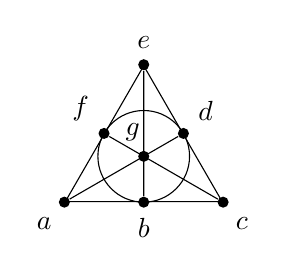
\begin{tikzpicture}[baseline=0]
    \node (tri) [draw,regular polygon,regular polygon sides=3,inner
    sep=0pt,minimum width=2.3cm] {};
    \node (e) [vertex,label={90:$e$}] at (tri.corner 1) {};
    \node (f) [vertex,label={150:$f$}] at ($(tri.corner 1)!0.5!(tri.corner 2)$) {};
    \node (a) [vertex,label={-120:$a$}] at (tri.corner 2) {};
    \node (b) [vertex,label={-90:$b$}] at ($(tri.corner 2)!0.5!(tri.corner 3)$) {};
    \node (c) [vertex,label={-60:$c$}] at (tri.corner 3) {};
    \node (d) [vertex,label={30:$d$}] at ($(tri.corner 3)!0.5!(tri.corner 1)$) {};
    \node (g) [vertex,label={[xshift=-4pt]90:$g$}] at (tri) {};
    \draw (a) -- (d) (e) -- (b) (c) -- (f);
    \node [draw] at (g) [circle through=(b)] {};
  \end{tikzpicture}\kern-2ex{ Fano-matroid,}
  $\FF_7^-=$\kern-2ex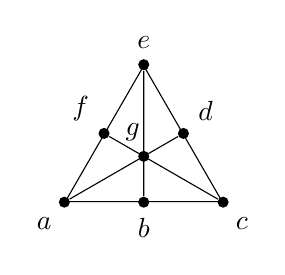
\begin{tikzpicture}[baseline=0]
    \node (tri) [draw,regular polygon,regular polygon sides=3,inner
    sep=0pt,minimum width=2.3cm] {};
    \node (e) [vertex,label={90:$e$}] at (tri.corner 1) {};
    \node (f) [vertex,label={150:$f$}] at ($(tri.corner 1)!0.5!(tri.corner 2)$) {};
    \node (a) [vertex,label={-120:$a$}] at (tri.corner 2) {};
    \node (b) [vertex,label={-90:$b$}] at ($(tri.corner 2)!0.5!(tri.corner 3)$) {};
    \node (c) [vertex,label={-60:$c$}] at (tri.corner 3) {};
    \node (d) [vertex,label={30:$d$}] at ($(tri.corner 3)!0.5!(tri.corner 1)$) {};
    \node (g) [vertex,label={[xshift=-4pt]90:$g$}] at (tri) {};
    \draw (a) -- (d) (e) -- (b) (c) -- (f);
  \end{tikzpicture}\kern-2ex{anti-Fano-matroid}
  + $\forall$ 4 elemű halmaz összefüggő, a 3 eleműek közül az egy
    egyenesre / körre esők
  + $\FF_7$ pontosan a $k = 2$ karakterisztikájú testek felett
    koordinátázható
  + $\FF_7^-$ pontosan a $k \ne 2$ karakterisztikájú
    testek felett koordinátázható
  + \proof $r(\FF_7) = r(\FF_7^-) = 3$ \RA feltehető: $a
    \mapsto (1, 0, 0)$, $c \mapsto (0, 1, 0)$, $e \mapsto (0, 0, 1)$
    + ekkor $b \mapsto (x, y, 0)$, $d \mapsto (0, z, u)$, $f \mapsto
      (v, 0, w)$, $g \mapsto (q, r, s)$
    + $\{ a, d, g \} \notin \FF$ \RA {\footnotesize$\begin{vmatrix}
        1 & 0 & q \\
        0 & z & r \\
        0 & u & s
      \end{vmatrix}$} $= 0$ \RA $sz = ru$; hasonlóan $sv = qw$, $rx =
    qy$
    + $\{ b, d, f \} \notin \FF(\FF_7)$, de $\in \FF(\FF_7^-)$ \RA%
      {\footnotesize$\begin{vmatrix}
        x & 0 & v \\
        y & z & 0 \\
        0 & u & w
      \end{vmatrix}$} $= 0$ $\FF_7$-ben, de $= 0$ $\FF_7^-$-ban
      + $wxz + uvy = 0$ $\FF_7$-ben, de $\ne$ $\FF_7^-$-ban
      + de $\frac{sz}{u} x = \frac{sv}{w} y$ \RA $swxz = suvy$ \RA%
        $wxz = uvy$
      + $wxz + wxz = 0$ $\FF_7$-ben pontosan akkor teljesül, ha $T$
        karakterisztikája $= 2$
      + $wxz + wxz \ne 0$ $\FF_7^-$-ban pontosan akkor teljesül, ha $T$
        karakterisztikája $\ne 2$ \qed
  + \corr az $\FF_7 \oplus \FF_7^-$ matroid nem lineáris
    + $T$ karakteriszikája egyszerre kellene $2$ és nem $2$ legyen
+ \example példák matroidokra
  \par
  {\centering\begin{tabular}{>{\footnotesize}l|l||>{\footnotesize}l|l}
    nem lineáris & $\FF_7 \oplus \FF_7^-$ &
    lineáris, de nem bináris & $\UU_{4, 2}, \FF_7^-$ \\\hline
    bináris, de nem reguláris & $\FF_7$ &
    reguláris, de nem grafikus & $\MM(K_5) \oplus [\MM(K_5)]^*$ \\\hline
    grafikus, de nem kografikus & $\MM(K_5)$ &
    kografikus, de nem grafikus & $[\MM(K_5)]^*$ \\\hline
    grafikus és kografikus & \multicolumn{3}{l}{$\MM(G)$, $G$ síkbarajzolható}
  \end{tabular}\par}
  + $K_5$ helyett tetszőleges nem síkbarajzolható gráf (pl.~$K_{3,3}$) állhat
+ \thm Tutte tételei
  + $\MM$ bináris \LRA nem minorja az $\UU_{4, 2}$
    + $\UU_{4, 2}$ rangja $2$, de $2$ dimenziós bináris vektorokból
      nem létezik $4$ db páronként lineárisan független;
      $\UU_{4, 2} = \MM \text{\footnotesize$\begin{pmatrix}
          1 & 0 & 1 & 1 \\
          0 & 1 & 1 & \mathbf{2}
        \end{pmatrix}$}$
  + $\MM$ reguláris \LRA nem minorja az $\UU_{4, 2}$,
  $\FF_7$ és $\FF_7^*$
  + $\MM$ grafikus \LRA nem minorja az $\UU_{4, 2}$,
    $\FF_7$, ${\FF_7^*}$, ${[\MM(K_5)]^*}$ és ${[\MM(K_{3, 3})]^*}$
    + ha $\MM(G)$ egy $G'$ gráf $[\MM(G')]^*$ vágásmatroidja, akkor
      $\MM(G)$ kografikus és $G'$ síkbarajzolható kell legyen
  + \noproof
+ \thm $\UU_{n, k}$ pontosan akkor grafikus, ha $k = 0, 1, n - 1$ vagy
  $n$
  + \proof $\UU_{n, 0}$ egy csúccsal és $n$ hurokkal reprezentálható,
    $\UU_{n, 1}$ $n$ párhuzamos éllel
  + $\UU_{n, n - 1}$ $n$ élű körrel reprezentálható, $\UU_{n, n}$ $n$
    elű erdővel
  + $\UU_{n, k} \setminus \{a\} = \UU_{n - 1, k}$, $\UU_{n, k} / \{a\}
    = \UU_{n - 1, k - 1}$
    + ha $2 \le k \le n - 2$ \RA $\UU_{n, k}$-nak van $\UU_{4, 2}$
      minorja
    + ehhez $n - k - 2$ törlés és $k - 2$ összehúzás kell \qed

\tetel{Matroidok összege. $k$-matroid-metszet probléma, ennek
  bonyolultsága $k \ge 3$ esetén.}

+ \dfn az $\MM_1 = (E, \FF_1), \MM_2 = (E, \FF_2), \ldots, \MM_k = (E,
  \FF_k)$ matroidok \emph{összeg}e az $\NN = \bigvee_{i = 1}^k \MM_i =
  (E, \FF')$ halmazrendszer, ahol
  $\FF' = \{ X_1 \cup X_2 \cup \ldots \cup X_k :  X_i \in \FF_i \; (i = 1, 2,
  \ldots, k) \}$
  + $\bigvee_{i = 1}^k (\MM_i \setminus X) = \bigl( \bigvee_{i = 1}^k
    \MM_i \bigr) \setminus X$, de az $/$ és a $\oplus$ műveletekre ez
    már nem igaz
+ \thm matroidok $\bigvee_{i = 1}^k \MM_i$ összege matroidot alkot
  + \proof $\MM_1 \vee (\MM_2 \vee \MM_3) = (\MM_1 \vee \MM_2) \vee
    \MM_3$ \RA elegendő $\MM_1 \vee \MM_2$-t vizsgálni
  + (F1): $\emptyset = \emptyset \cup \emptyset \in \FF_1 \vee \FF_2$
  + (F2): $X = X_1 \cup X_2$, $X_1 \in \FF_1$, $X_2 \in \FF_2$, $Y
    \subseteq X$
    + ekkor $X_1 \supseteq Y \cap X_2 \in \FF_1$, $X_2
      \supseteq Y \cap X_2 \in \FF_2$, $(Y \cap X_2) \cup (Y \cap X_2) =
      Y \in \FF'$
  + (F3): legyen $X, Y \in \FF'$; $\lvert X \rvert > \lvert Y \rvert$;
    $X = X_1 \cup X_2$; $Y = Y_1 \cup Y_2$; $X_1, X_2 \in \FF_1$; $Y_1,
    Y_2 \in \FF_2$
    + ált.~megsz.~nélkül~tfh.~$\rvert X_1 \cap Y_2 \lvert +
      \lvert X_2 \cap Y_1 \rvert$ minimális, $X_1 \cap X_2 = Y_1 \cap
      Y_2 = \emptyset$
    + ált.~megsz.~nélkül~tfh.~$\lvert X_1 \rvert > \lvert Y_1 \rvert$
      \RA $\exists e \in X_1 - Y_1 : Y_1 \cup \{ e \} \in \FF_1 \subseteq \FF_1$
    + ha $e \notin Y_2$ \RA $e \in X - Y$, $Y \cup \{ e \} = (Y_1 \cup \{e\}) \cup
      Y_2 \in \FF'$
    + ha $e \in Y_2$ \RA $Y = Y_1' \cup Y_2' = (Y_1 \cup \{e \})
      \cap (Y_2 - \{e \})$ is egy jó felbontása $Y$-nak
      + vegyük észre, hogy $X_1 \cap X_2 = \emptyset$, $e \in X_1$ \RA $e \notin X_2$
      + $\rvert X_1 \cap (Y_2 - \{e\}) \lvert + \lvert X_2 \cap (Y_1
        \cup \{e\}) \rvert = \rvert X_1 \cap Y_2 \lvert - 1 + \lvert X_2
        \cap Y_1 \rvert$
      + a metszetek méretének összege nem lehetett minimális,
        ellentmondás \qed
+ \dfn az $\MM_1 = (E, \FF_1), \MM_2 = (E, \FF_2), \ldots, \MM_k = (E,
  \FF_k)$ matroidok \emph{metszet}e az $(E, \FF')$ halmazrendszer, ahol
  $\FF' = \bigcap_{i = 1}^k \FF_i$
  + ez nem mindig matroid, pl.~%
  $\MM\mleft(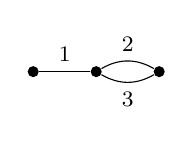
\begin{tikzpicture}[baseline=-.5ex,font=\footnotesize]
    \node (a) [vertex] at (0,0) {};
    \node (b) [vertex] at (0.8,0) {};
    \node (c) [vertex] at (1.6,0) {};
    \draw (a) edge node [above] {1} (b);
    \draw (b) edge [bend left] node [above] {2} (c);
    \draw (b) edge [bend right] node [below] {3} (c);
  \end{tikzpicture}\mright)$ és
  $\MM\mleft(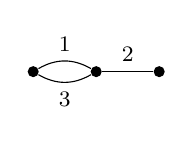
\begin{tikzpicture}[baseline=-.5ex,font=\footnotesize]
    \node (a) [vertex] at (0,0) {};
    \node (b) [vertex] at (0.8,0) {};
    \node (c) [vertex] at (1.6,0) {};
    \draw (b) edge node [above] {2} (c);
    \draw (a) edge [bend left] node [above] {1} (b);
    \draw (a) edge [bend right] node [below] {3} (b);
  \end{tikzpicture}\mright)$
  metszete nem az, mert $\FF' = \{ \emptyset, \{1\}, \{2\}, \{3\},
    \{2, 3\}\}$ \RA (F3) nem teljesül
+ \prob (súlyozott) $k$-matroid metszet ($k$-MMP)
  + \DataIn $\MM_1 = (E, \FF_1), \MM_2 = (E, \FF_2), \ldots, \MM_k = (E,
    \FF_k)$, $p \in \Nat$ ($w\colon E \to \RR_{\ge 0}$, $W \in \RR_{\ge 0}$)
  + \DataOut $\exists$-e olyan $X \in \bigcap_{i = 1}^k \FF_i$, hogy
    $\lvert X \rvert \ge p$ (illetve $w(X) \ge W$)
+ \thm $k \ge 3$ esetén $k$-MMP NP-nehéz
  + \proof $3$-MPP NP-nehéz \RA $k > 3$, $k$-MMP NP-nehéz
    + adunk egy $3$-MMP $\prec$ $k$-MMP Karp-redukciót ($k > 3$)
    + $(\MM_1, \MM_2, \MM_3) \in \text{$3$-MPP}$ \LRA $(\MM_1, \MM_2,
      \overbrace{\MM_3, \MM_3, \ldots, \MM_3}^{\text{$k - 2$ db}}) \in
      \text{$k$-MPP}$
  + irányított $s$-$t$-HAMÚT $\prec$ $3$-MMP \RA $3$-MPP NP-teljes
    + $\MM_1 = \MM(G)$
    + $\FF(\MM_2) =$ azon élhalmazok, melyekben $\forall$ pont be-foka
      $\le 1$, $d_{\text{be}}(s) = 0$
      + egy partíció-matroidból kapjuk $s$ bemenő éleinek összehúzásával
    + $\FF(\MM_3) =$ azon élhalmazok, melyekben $\forall$ pont
      \rlap{ki-foka}\phantom{be-foka} $\le 1$,
      $d_{\text{\rlap{ki}\phantom{be}}}(\mathrlap{t}\phantom{s}) = 0$
    + $p = \lvert V \rvert - 1$ \RA $X \in \FF_1, \FF_2, \FF_3$;
      $\lvert X \rvert \ge p$ épp $s$-$t$ Hamilton-út \qed

\tetel{A $k$-matroid partíciós probléma, ennek algoritmikus
  megoldása. A $2$-matroid-metszet feladat visszavezetése matroid
  partíciós problémára.}

+ \prob $k$-matroid partíció ($k$-MPP)
  + \DataIn $\MM_1 = (E, \FF_1), \MM_2 = (E, \FF_2), \ldots, \MM_k = (E,
    \FF_k)$
  + \DataOut $E$ független-e $\bigvee_{i = 1}^k \MM_i$-ben? \LRA
    $\bigvee_{i = 1}^k \MM_i \overset{?}{=} (E, 2^E)$
    + \LRA $\overset{?}{\exists} E_1 \in \FF_1, E_2 \in \FF_2, \ldots,
      E_k \in \FF_k : E = E_1 \cup E_2 \cup \ldots \cup E_k$
+ \alg $k$-matroid partíció algoritmus\footnote{Edmonds, J.~és
  D.~R.~Fulkerson (1965). Transversals and Matroid Partition. In:
  \emph{J.~OF~RESEARCH of the Nat.~Bureau of Standards---B.~Math.~and
    Math.~Phys.~Vol.~69B, No.~3}}
  + 0.~lépés: $E_1 \gets \emptyset$, $E_2 \gets \emptyset$, \ldots,
    $E_k \gets \emptyset$
  + 1.~lépés ha $\bigcup_{i = 1}^k E_i = E$ \RA STOP, igaz
  + 2.~lépés van-e $x \in E - \bigcup_{i = 1}^k E_i$, hogy
    $\bigcup_{i = 1}^k E_i \cup \{x\}$-t partícionálható?
    + ha igen \RA legyen $E_1, E_2, \ldots E_k$ az új partícionálás,
      GOTO 1.
    + ha nem \RA STOP, hamis
  + irányított $\vec{G} = (V, \vec{E})$ segédgráf konstrukció a
    2.~lépés elvégzéséhez
    + $V = E \cup P = E \cup \{ p_1, p_2, \ldots, p_k\}$
    + $(a, p_i) \in \vec{E}$ \LRA $a \notin E_i$, de $E_i \cup \{a\}
      \in \FF_i$
    + $(a, b) \in \vec{E}$ \LRA valamely $i$-re $b \in E_i$, $a \notin
      E_i$, $E_i \cup \{a\} \notin \FF_i$, $E_i \cup \{a\} - \{b\} \in
      \FF_i$
  + szélésségi kereséssel keressük meg a legrövidebb utat $E' = E -
    \bigcup_{i = 1}^k E_i$-ből $P$-be
    + van \RA $(a, b)$-kre $b \in E_i$ esetén $E_i \gets
      E_i \cup \{a\} - \{b\}$; $(a, p_i)$-re $E_i \gets E_i
      \cup \{a\}$
      + $\vec{G}$ definíciója miatt még $\forall E_i \in
        \FF_i$; $E'$ mérete $1$-gyel (út első csúcsa) nőtt
    + nincs \RA legyen $X \subset E$ az $E'$-ből irányított úton
      elérhető csúcsok halmaza
      + $r(X) \le \sum_{i = 1}^k r_i(X) < \lvert X \rvert$ \RA $E
        \supset X \notin \bigcup_{i = 1}^k \FF_i$
        $\xRightarrow{\text{(F2)}}$ $E$ nem lehet
        független
  + lépésszám: $O(\lvert E \rvert + \overbrace{c (n +
    k)^2}^{\text{gráf}} + \overbrace{c (n +
    k)^2}^{\text{szélességi}})$
+ \thm az $\MM_1 = (E, \FF_1)$ és $M_2 = (E, \FF_2)$ azonos rangú
  ($r_1(E) = r_2(E)$) matroidoknak pontosan akkor van közös bázisa, ha
  $\MM_1 \vee \MM_2^* = (E, 2^E)$
  + (\RA) ha $B$ közös bázis, akkor $E - X$ bázisa $\MM_2^*$-nak
    + $E = X \cup (E - X)$ független az összegben \RA $\MM_1 \vee
      \MM_2^*$ teljes
  + (\LA) legyen $E = E_1 \cup E_2$, $E_1 \in \FF_1$, $E_2 \in
    \FF_2^*$
    + $\lvert E \rvert \le \lvert E_1 \rvert + \lvert E_2 \rvert =
      r_1(E_1) + r_2^* (E_2) = r_1(E_1) + (\lvert E \rvert - r_2(E) +
      r_2(E - E_2)) \le\\\phantom{\lvert E \rvert}\le r_1(E) + (\lvert E
      \rvert - r_2(E)) = \lvert E \rvert$
    + mindenhol egyenlőség kell álljon, tehát $\lvert E \rvert \le
    \lvert E_1 \rvert + \lvert E_2 \rvert$ \RA $E_1 = E - E_2$
    + $r_1(E_1) = r_1(E)$, $r_2(E) = r_2(E - E_2) = r_2(E_1)$ \RA%
      $E_1$ közös bázis \qed
+ \corr $2$-MMP visszavezetése $2$-MPP
  + legyen $\MM_1' = (E, \FF_1')$,  $\MM_2' = (E, \FF_2')$, ahol
    $\FF_i' = \{ X \in \FF_i : \lvert X \rvert \le p \}$ a matroidok
    \emph{csonkoltjai}
  + $\forall$ $p$ méretű független halmaz bázis a megfelelő csonkolt
    matroidban
  + $\MM_1' \vee (\MM_2')^* = (E, 2^E)$ \LRA $\MM_1'$-nek és
    $\MM_2'$-nek van közös bázisa
  + ez a bázis a $2$-MMP-ben keresett $p$ méretű közös
  független halmaz $\MM_1$-ben és $\MM_2$-ben

\tetel{$k$-polimatroid rangfüggvény fogalma. A
  $2$-polimatroid-matching probléma, ennek bonyolultsága, Lovász
  tétele (biz.~nélkül).}

+ \dfn $r\colon 2^E \to \Nat$ \emph{$k$-polimatroid rangfüggvény}, ha
  + (R1)~$r(\emptyset) = 0$\qquad(R2$'$)~$\forall e \in E : r(\{e\})
    \le k$\qquad(R3)~$Y \subseteq X \implies r(Y) \le r(X)$
  + (R4)~$r(X) + r(Y) \ge r(X \cap Y) + r(X \cup Y)$
  + a matroid rangfüggvények $k = 1$ választással adódnak
    + $X = \{e_1\} \cup \{e_2\} \cup \ldots \cup \{e_m\}$
      $\xRightarrow{\text{(R4)}}$ $m \le \sum_{i = 1}^m r(\{e_i\}) \le
      r(X)$
  + másik irány: $\forall X \subseteq E : r(X) \le k \lvert X \rvert$
+ \dfn $X \subseteq E$ egy $k$-matching, ha $r(X) = k \lvert X \rvert$
+ \example $G = (V, E)$ gráf, $r(X) =$ az $X \subseteq E$ élek által
  lefedett csúcsok halmaza
  + $r$ egy $2$-polimatroid-rangfüggvény, a $2$-matchingek $G$
    párosításai
+ \prob $k$-polimatroid matching ($k$-PMMP)
  + \DataIn $r\colon 2^E \to \Nat$ $k$-polimatroid rangfüggvény, $p
    \in \Nat$
  + \DataOut létezik-e $X \subseteq E$, hogy $r(X) = k \lvert X
    \rvert$ és $\lvert X \rvert \ge p$
+ \thm a $k$-PMMP $k \ge 3$ esetén NP-nehéz
  + \proof $k$-MMP $\prec$ $k$-PMMP és $k$-MMP NP-nehéz
  + ha $\MM_1, \MM_2, \ldots, \MM_k$ matroidok \RA $r(X) = \sum_{i =
    1}^k r_i(X)$ $k$-polimatroid rangfüggvény
    + a $k$-matchingek pontosan a  független halmazok $\forall \MM_i$-ben
    + $(\MM_1, \MM_2, \ldots, \MM_k; p) \in \text{$k$-MMP}$ \LRA%
      $\bigl(\sum_{i = 1}^k r_i, p\bigr) \in \text{$k$-PMMP}$ \qed
+ \thm ha $r$ mindössze egy $O(1)$ időben kiszámolható orákulummal
  adott \RA\\$2$-PMMP nem oldható meg polinomidőben
  + \proof legyen $\lvert E \rvert = 2n$, $E_0 \subset E$, $\lvert E_0
    \rvert = n$
  + $r_1(X) \coloneqq \text{\footnotesize$\begin{cases}
      2 \lvert X \rvert, &\text{ha $\lvert X \rvert < n$,} \\
      2n - 1, &\text{ha $\lvert X \rvert = n$,} \\
      2n, &\text{ha $\lvert X \rvert > n$,}
    \end{cases}$}$ $r_2(X) \coloneqq \text{\footnotesize$\begin{cases}
      2 \lvert X \rvert, &\text{ha $\lvert X \rvert < n$,} \\
      2n, &\text{ha $X = E_0$,} \\
      2n - 1, &\text{ha $X \ne E_0, \lvert X \rvert = n$,} \\
      2n, &\text{ha $\lvert X \rvert > n$,}
    \end{cases}$}$ $p \coloneqq n$
  + $(r_1, p) \notin \text{$2$-PMMP}$, de $(r_2, p) \in
    \text{$2$-PMMP}$ ($E_0$ egy $p = n$ elemű $k$-matching)
    + ennek eldöntéséhez az összes $n$ elemű részhalmazt meg kell vizsgálni
    + ez $\binom{2n}{n} = O(4^n / \sqrt{\pi n})$ darab $r$ hívást igényel \qed
  + nem használtuk ki, hogy $2$-PMMP NP-nehéz, a bizonyítás P = NP
    esetén is működik
+ \thm (Lovász László tétele)
  + ha az $r$ $2$-polimatroid rangfüggvény
    $r(X) = \operatorname{dim} \bigl\langle \bigcup_{i \in X} \{ a_i, b_i
    \} \bigr\rangle$ alakban adott, ahol $E = \{1, 2, \ldots, n\}$,
    $\{a_i, b_i\}_{i \in I} \subset \RR^k$
    \RA $r$-en $2$-PMMP polinomidőben megoldható
  + az ilyen $r$ mindig $2$-polimatroid rangfüggvény
  + \noproof


\section{Közelítő és ütemezési algoritmusok} 

\tetel{Polinomiális időben megoldható feladat fogalma, példák. Az NP,
  co-NP, NP-nehéz és NP-teljes problémaosztályok definíciója,
  viszonyaik, példák problémákra valamennyi osztályból. NP-nehéz
  feladatok polinomiális speciális esetei: algoritmus a maximális
  független ponthalmaz problémára és az élszínezési problémára páros
  gráfokon. Additív hibával közelítő algoritmusok speciális pont-,
  illetve élszínezési problémákra.}

+ algoritmuselméleti alapfogalmak
  + \dfn \emph{kiszámítási problémá}ról akkor beszélünk, ha egy $I$
    bemenet $f(I)$ függvényét szeretnénk kimenetként megadni
    + \emph{eldöntési probléma}: $f(I) \in \{\textsc{Igen},
      \textsc{Nem}\}$
  + \dfn \emph{optimalizálási probléma} olyan kiszámítási probléma, ahol
    + az $I$ bemenethez $X_I$ a \emph{lehetséges kimenetek} halmaza,
      $c\colon X_I \to \RR$ valós függvény
    + $f(I) = x^* \in X_I$, hogy $c(x^*) = \max \{ c(x) : x \in X_I \}$
      (illetve $c(x^*) = \min \{ c(x) : x \in X_I \}$)
    + a kimenet nemcsak az optimum értéke, hanem maga az $x^*$ optimális
      megoldás
  + \dfn egy $f \colon \Nat \to \Nat$ függvény \emph{polinomális}, ha
    $\exists c_1, c_2 \in \Nat^*: \forall n \in \Nat : f(n) \le c_1
    n^{c_2}$
    + egy algoritmus akkor \emph{polinomiális} ha $\forall$ $n$ méretű
      bemenetre $f(n)$ időben kiszámítja a kimenetet, ahol $f$
      polinomiális
    + egy probléma \emph{polinom időben megoldható}, ha $\exists$ rá
      polinomiális algoritmus
  + \dfn az $A$ probléma \emph{polinom időben visszavezethető} $B$-re
    ($A \cookprec B$), ha $A$ polinom időben megoldható a
    $B$-t megoldó algoritmus szubrutinként hívásával
    + $B$ hivása $O(1)$ lépésnek számit
  + \dfn döntési problémák osztályai
    + P $\coloneqq$ a polinom időben megoldható eldöntési
      problémák osztálya
      + pl.~teljes párosítás páros gráfban, $k$-matroid-partíció
    + NP $\coloneqq$ azon eldöntési problémák osztálya, ahol az
      \textsc{Igen} válaszra létezik polinomiális méretű, polinomiális
      időben ellenőrizhető tanú
      + pl.~Hamilton-kör, $k$-matroid-metszet ($k \ge 2$)
    + co-NP $\coloneqq$ azon eldöntési problémák osztálya, ahol az
      \textsc{Nem} válaszra létezik polinomiális méretű, polinomiális
      időben ellenőrizhető tanú
      + pl.~teljes párosítás páros gráfban (Kőnig tétele, Hall-tétel),
        síkbarajzolhatóság (Kuratowski-tétel), teljes párosítás
        tetszőleges gráfban (Tutte-tétel)
    + egy $B$ probléma \emph{NP-nehéz}, ha $\forall A \in
      \mathrm{NP}: A \cookprec B$
      + pl.~az általános $k$-polimatroid matching NP-nehéz, de nem
        NP-beli
    + egy $B$ probléma \emph{NP-teljes}, ha NP-beli és NP-nehéz
      + pl.~SAT (Cook`--Levin tétel), 3SZÍN, HAM, LÁDAPAKOLÁS
  + P $\subseteq$ NP $\cap$ co-NP, NP-teljes $=$ NP $\cap$ NP-nehéz, P
    $\overset{?}{=}$ NP
+ \prob maximális független ponthalmaz páros gráfban
  + \DataIn $G = (A, B; E)$ páros gráf\qquad\DataOut $F$ maximális
    független ponthalmaz
  + a probléma általános gráfra NP-nehéz, de páros gráfra polinomiális
  + futtasuk le a gráfra a javítóutas algoritmust (polinom idejű)
  + \stmnt ekkor $F = A_1 \cup A_2 \cup B_1 \cup B_3$ maximális
    független ponthalmaz
    + $A_1, B_1 =$ az $A$-, illetve $B$-beli párosítatlan pontok
      halmaza
    + $B_2 =$ az $A_1$-ből alternáló úton elérhető pontok (nincs
      javító út \RA mind van párjuk)
    + $A_1 =$ a $B_2$-beli pontok párjai
    + $A_3 = A - A_1 - A_2$, $B_3 = B - B_1 - B_2$
    + \proof az algoritmus által megtalált $M$ párosítás maximális \RA%
      $\lvert M \rvert = \nu(G)$
      + $\nu(G) =$ maximális párosítás mérete, $\tau(G) =$ min.~lefogó
        ponthalmaz mérete
      + nincs él $A_1 \cup A_2$ és $B_1 \cup B_2$ között
        (\ref{thm:linprog:egervary:magyar}.~tétel) \RA $F$ független
      + $A \cup B - F = A_3 \cup B_2$ lefogó ponthalmaz \RA $\tau(G)
        \le \lvert A_3 \cup B_2 \rvert = \lvert F \rvert = \nu(G)$
      + egy lefogó ponthalmaz egy párosítás $\forall$ élét le kell
        fogja \RA $\nu(G) \le \tau(G)$
      + így $\tau(G) \le \lvert A_3 \cup B_2 \rvert = \lvert F \rvert
        = \nu(G) \le \tau(G)$ \RA $\nu(G) = \tau(G)$
    + indir.~tfh.~$\exists F' \subseteq A \cup B$ független
      ponthalmaz, $\lvert F' \rvert > \lvert F \rvert$
      + ekkor $A \cup B - F'$ lefogó ponthalmaz, de $\lvert A \cup B -
        F' \rvert < \lvert A \cup B - F \rvert = \tau(G)$
      + ez ellentmondás, $F$ maximális kell legyen \qed
+ \prob élszínezés páros gráfokon
  + \DataIn $G = (A, B; E)$ egyszerű páros gráf\qquad\DataOut $G$ élszínezése
    $\Delta(G)$ színnel
  + a probléma általános gráfra NP-nehéz, de páros gráfra polinomiális
  + \thm \label{thm:kozelito:additiv:vizing}(Vizing tétele) ha $G = (V, E)$ egyszerű gráf \RA $\Delta(G)
    \le \chi_e(G) \le \Delta(G) + 1$
    + \noproof
  + \thm (Kőnig tétele) ha $G = (A, B; E)$ egyszerű páros gráf \RA%
    $\chi_e(G) = \Delta(G)$
    + \proof meg fogunk adni egy polinomiális algoritmust a színezésre
  + vegyük a gráf $E = \{ e_1, e_2, \ldots, e_m \}$ éleit sorban, és
    színezzük meg őket egy-egy szabad színnel
    + legyen $e_i = \{u, v\}$, $ u \in A$, $v \in b$ a most
      megszínezendő él
    + $d(u), d(v) \le \Delta(G)$, és illeszkedik rájuk színezetlen él
      ($e_i$)
      + \RA mindkét csúcsnak $\exists$ szabad színe \RA ha $\exists$
      közös szabad szín, $e_i$ kapja meg azt
  + tfh.~az $u$ szabad színe a \emph{piros}, de a $v$-é a \emph{kék}
    + legyen $P_u$ az $u$-ból induló, felváltva kék--piros út (kör nem
      lehet)
    + ekkor $v \notin P_u$, mert akkor a végpontja lenne ($v$-ben a
      kék szabad)
      + de $u \in A$, $v \in B$ \RA $P_u$ páratlan hosszú \RA $P_u$
        utolsó éle kék
    + cseréljük fel $P_u$ mentén a piros és a kék színeket
      + ez a meglevő színezést nem ronthatja el
      + $u$-ban most már a kék szabad, $v$-ben maradt szabad \RA%
        $e_i$ színezhető kékre \qed
+ \dfn egy maximalizálási (minimalizálási) problémát egy algoritmus
  \emph{$C$ additív hibától eltekintve helyesen old meg}, ha $\forall I:
  c(x^*) \ge \max_{x \in X_i} c(x) - C$ ($c(x^*) \le \min_{x \in X_i}
  c(x) + C$)
+ \dfn egy algoritmus \emph{$C$ additív hibával közelítő algoritmus},
  ha adott optimalizálási problémát polinom időben, $C$ additív
  hibától eltekintve helyesen old meg
+ \prob egyszerű gráfok élszínezése
  + \DataIn $G = (V; E)$ egyszerű gráf\qquad\DataOut $G$
    minimális élszínezése
  + Vizing tétele (\ref{thm:kozelito:additiv:vizing}.~tétel) szerint
    $\chi_e(G) \le \Delta(G) + 1$
    + a tétel bizonyítása konstruktív, ad egy $\Delta(G) + 1$ polinom
      időben
    + így a tételben szereplő algoritmus $1$ additív hibával közelítő
+ \prob síkgráfok csúcsszínezése
  + \DataIn $G = (V; E)$ síkgráf\qquad\DataOut $G$
    minimális csúcsszínezése
  + \thm (négyszíntétel) minden síkgráf színezhető $4$ színnel,
    \noproof
    + létezik algoritmikus bizonyítás, ami polinomidőben előállít egy
      $4$-színezést
    + ez egy $2$ additív hibával közelítő algoritmus
  + ha a $4$-színező algoritmus előtt ellenőrizzük, hogy $G$ páros-e
    \RA $2$-színezhető
    + ez szélességi kereséssel polinomidőben megtehető

\tetel{A Hamilton-kör probléma visszavezetése a leghosszabb kör
  probléma additív közelítésére. $k$-approximációs algoritmus fogalma,
  példák: két-két algoritmus a minimális lefogó ponthalmaz keresésére
  és a maximális páros részgráf keresésére. Minimális levelű, illetve
  maximális belső csúcsú feszítőfa keresése. Approximációs algoritmus
  az utóbbi feladatra (biz.~nélkül).}

+ \prob leghosszabb kör (LHK)
  + \DataIn $G = (V, E)$ gráf\qquad\DataOut $G$ egy leghosszabb köre
  + \thm ha P $\ne$ NP \RA LHK-re nincs $C$ additív hibával
    közelítő algoritmus
    + \proof megmutatjuk, hogy HAM $\prec$ LHK $C$-additív közelítése
    + indir.~tfh.~$\exists$ $C$-additív hibájú közelítés LHK-ra
    + $G' \coloneqq$ osszuk fel a $G$ gráf $\forall$ élét $C$ új
      ponttal \RA egy él helyett $C + 1$ új él
    + $G'$ $k (C + 1)$ hosszú körei $G$ $k$ hosszú köreinek felelnek meg
    + $G'$-ben van $n (C + 1)$ hosszú kör \LRA $G$-ben van $n$ hosszú
      kör \LRA $G$ hamiltoni
    + $G$ hamiltoni \RA a közelítő algoritmus $\ge n (C + 1) - C$
      hosszú $x^*$ kört talál $G'$-ben
      + de $G'$ köreinek hossza osztható $(C + 1)$-gyel \RA $x^*$
        csak a Hamilton-kör lehet \qed
+ \dfn egy maximalizálás (minimalizálási) problémát egy algoritmus
  \emph{$k$ multiplikatív hibától eltekintve helyesen old meg}, ha
  $\forall I : c(x^*) \ge \frac{1}{k} \max_{x \in X_I} c(x)$
  ($c(x^*) \le k \min_{x \in X_I} c(x)$)
+ \dfn egy algoritmus \emph{$k$-approximációs algoritmus}, ha
  polinomiális és $k$ multiplikatív hibától eltekintve helyesen oldja
  meg az adott problémát
+ \prob minimális lefogó ponthalmaz (MLP)
  + \DataIn $G = (V, E)$\qquad\DataOut egy $X$ minimális lefogó ponthalmaz
    $G$-ben
  + MLP NP-nehéz, mert a maximális független halmaz (MFP) is az, és
    MFP $\prec$ MFP
    + $X$ minimális független ponthalmaz \LRA $V - X$ maximális lefogó
      ponthalmaz
    + az MFP nem $k$-approximálható (\noproof)
  + \alg $2$-közelítő algoritmus maximális párosítással
    + 1.~lépés: keressük meg $G$ egy $M$ maximális párosítását
      + páros gráfban: magyar modszer, általános gráfban: Edmonds
        algoritmusa
    + 2.~lépés $X \coloneqq$ az $M$-beli élek végpontjai
    + \thm \label{thm:kozelito:multi:lefogo1}az így meghatározott $X$-re $\lvert X \rvert \le 2 \tau(G)$
      + \proof egy lefogó ponthalmaz $M$ $\forall$ élét le kell fogja
        \RA $\lvert M \rvert = \nu(G) \le \tau(G)$
      + $\lvert F \rvert = 2 \lvert M \rvert = 2 \nu(G) \le 2 \tau(G)$
        \qed
  + \alg $2$-közelítő algoritmus tovább nem bővíthető párosítással
    + 0.~lépés: $M \coloneqq \emptyset$
    + 1.~lépés: ha van olyan $e \in E$, hogy $M \cup \{e\}$ párosítás
      \RA $M \gets M \cup \{e\}$, GOTO 1.
      + egyébként $M$ egy tovább nem bővíthető párosítás
    + 2.~lépés: $X \coloneqq$ az $M$-beli élek végpontjai
    + \thm az így meghatározott $X$-re $\lvert X \rvert \le 2 \tau(G)$
      + \proof \aref{thm:kozelito:multi:lefogo1}.~tételben nem
        használtuk ki, hogy $M$ maximális
      + így továbbra is $\lvert F \rvert = 2 \lvert M \rvert \le 2
        \nu(G) \le 2 \tau(G)$ \qed
  + éles példa: $m$ darab diszjunkt $1$ hosszú út
    + optimális megoldás: mindegyik élnek csak az egyik végét vesszük
      bele \RA $m$ csúcs
    + közelítő megoldás: mindegyik él mindkét vége \RA $2m$ csúcs
+ \prob maximális páros részgráf (MPR) \RA NP-nehéz (\noproof)
    + \DataIn $G = (V, E)$ gráf
    + $A, B: A \cup B = G, A \cap B = \emptyset$, az $A$ és $B$ között
      menő élek száma maximális
    + \alg \label{alg:kozelito:multi:paros1}$2$-approximációs algoritmus 1.
      + 1.~lépés: osszuk ketté a csúcshalmazat $A$-ra és $B$-re
        tetszőlegesen
      + $d_{\mathrlap{s}\phantom{m}}(v) \coloneqq$ $v$-ből a saját
        csoportjába menő élek száma
      + $d_m(v) \coloneqq$ $v$-ből a másik csoportba menő élek száma
      + 2.~lépés: keressünk egy olyan $v$ csúcsot, amire $d_s(v) >
        d_m(v)$
        + ha van ilyen $v$, helyezzük át a másik csoportba; GOTO 2.
      + 3.~lépés: $(A, B)$ egy $2$-approximáció az MPR problémára
      + \thm \label{thm:kozelito:multi:paros1}az így meghatározott $(A, B)$ valóban $2$-approximáció
        + \proof $\forall$ lépésben az $A$ és $B$ között haladó élek
          száma nő \RA $\le \lvert E \rvert$ lépés
        + $\forall v \in V : d_m(v) \ge d_s(v)$ \RA $\frac{1}{2}
          \sum_{v \in V} d_m(v) \ge \frac{1}{2} \sum_{v \in V} d_s(v)$
        + $\frac{1}{2} \sum_{v \in V} d_m(v)$ az $A$ és $B$ között
          menő élek száma
        + $\frac{1}{2} \sum_{v \in V} d_m(v) = \frac{1}{4} \sum_{v
          \in V} d_m(v) + d_m(v) \ge \frac{1}{4} \sum_{v \in V}
          d_m(v) + d_s(v) = \frac{1}{2} \lvert E \rvert \ge
          \frac{1}{2} \lvert E_{\max} \rvert$,
          ahol $E_{\max} \subseteq E$ a maximális páros részgráf
          éleinek halmaza \qed
    + \alg $2$-approximációs algoritmus 2.
      + 1.~lépés $A \coloneqq \emptyset$, $B \coloneqq \emptyset$
      + 2.~lépés $G$ pontjait valamilyen sorrendben véve helyezzük el
        azoka a halmazokba, ahol \emph{kevesebb} szomszédjuk van
      + \thm az így meghatározott $(A, B)$ valóban $2$-approximáció
        + továbbra is igaz az, hogy $\forall v \in V : d_m(v) \ge
        d_s(v)$ \RA lásd \aref{thm:kozelito:multi:paros1}.~tételt \qed
      + jobb közelítéshez (ha szerencsénk van) még futtathatjuk
        \aref{alg:kozelito:multi:paros1}.~algoritmust
+ \prob minimális levelű feszítőfa (MLF)
  + \DataIn $G = (V, E)$ összefüggő gráf
  + \DataOut $F$ minimális számú $1$ fokú csúcsot tartalmazó feszítőfa
    $G$-ben
  + \thm MLF NP-nehéz
    + \proof HAMÚT $\prec$ MLF
      + a Hamilton-út $2$ levelű feszítőfa, ennél kevesebb levelű
        pedig nem létezhet \qed
    + MLF-re nem létezik $k$-approximációs algoritmus (\noproof)
+ \prob maximális belső csúcsú feszítőfa (MBF)
  + \DataIn $G = (V, E)$ összefüggő gráf
  + \DataOut $F$ maximális számú \emph{nem} $1$ fokú csúcsot
    tartalmazó feszítőfa $G$-ben
  + MBF ekvivalens MLF-fel, ezért szintén NP-nehéz, de már
    $k$-approximálható
  + \alg $2$-appriximációs algorimus MBF-re
    + ILST = Independent Leaves Spanning Tree
    + 0.~lépés: legyen $F$ egy tetszőleges feszítőfa $G$-ben
    + 1.~lépés: ha $F$ Hamilton-út, vagy a levelei független halmazt
      alkotnak \RA STOP
    + 2.~lépés: legyen $a$ és $b$ $F$ két levele, ahol $\{a, b\} \in E$
      (szomszédosak $G$-ben)
      + keressük meg a $P = a \leadsto b$ (egyértelmű) utat $F$-ben
      + $F$ nem Hamilton-út \RA $P$-nek van $F$-ben $\ge 3$.~fokú
        csúcsa \RA az egyik legyen $v$
    + 3.~lépés: legyen $w : \{v, w\} \in B$, $F \gets F - \{\{v, w\}\}
      \cup \{\{a, b\}\}$, GOTO 1.
      + az így kapott $F$ továbbra is feszítőfa, a levelek száma
      csökkent
    + \thm a fenti algoritmus polinomiális, $F$ egy $2$-approximáció
      MBF-re
      + \noproof
  + \alg $2$-appriximációs algorimus MBF-re mélységi kereséssel
    + 1.~lépés: legyen $F$ a $G$ mélységi feszítőfája $r \in E$-ből
      indítva
    + 2.~lépés: ha $F$ Hamilton-út, vagy $d(r) > 1$ \RA STOP
      + ha $d(r) = 1$, de $r$ nem szomszédos $F$ másik levelével \RA
      STOP
    + 3.~lépés: legyen $a$ olyan levele $F$-nek, mellyel $r$
    szomszédos
      + keressük meg a $P = r \leadsto a$ utat $F$-ben (egyértelmű)
      + $v$ az $a$-hoz legközelebbi $\ge 3$.~fokú csúcs $P$-ben
      + $w$ a $v$-vel szomszédos csúcs a $v \leadsto a$ úton $P$-ben
        (lehet, hogy $w = a$)
    + 4.~lépés: $F \gets F - \{\{v, w\}\} \cup \{\{r, a\}\}$
    + \thm a fenti algoritmus $O(\lvert E \rvert)$ idejű, $F$ egy $2$-approximáció
      MBF-re
      + \noproof   

\tetel{A minimális lefogó ponthalmaz probléma visszavezetése a
  halmazfedési feladatra, a halmazfedési feladat közelítése, éles
  példa. Közelítő algoritmus a Steiner-fa problémára, éles példa.}

+ \prob súlyozott halmazfedés (SHF)
  + \DataIn $n$ elemű $U$ alaphalmaz, $\CR \subseteq 2^U : \bigcup_{S
    \in \CR} S = U$, $c\colon \CR \to \QQ^+$ költségfüggvény
  + \DataOut $\CR' \subseteq \CR$, ahol $\bigcup_{S \in \CR'} S = U$
    és $\sum_{S \in \CR'} c(S)$ minimális
  + \thm a súlyozott halmazfedés probléma NP-nehéz
    + \proof megmutatjuk, hogy MLP $\prec$ SHF
    + keressük a $G = (V, E)$ gráf minimális lefogó ponthalmazát
    + $U \coloneqq E$, $\CR \coloneqq \{E_v = \{e : u \in V, e = \{v,
      u\} \in E\} : v \in V\}$, $c(E_v) \coloneqq 1$
    + $\CR'$ minimális fedés \LRA $F \subseteq V$ min.~lefogó
      ponthalmaz, ahol $\CR' = \{ E_v : v \in \CR'\}$ \qed
  + \thm ha P $\ne$ NP \RA $\nexists$ konstants $k$-faktorú
    approximáció SHF-re (\noproof)
  + \alg Chvátal mohó algoritmusa
    + 0.~lépés: $\CR' \coloneqq \emptyset$, $C \coloneqq \emptyset$ a már
      lefedett elemek halmaza
    + 1.~lépés: ha $C = U$ \RA STOP, egyébként $S = \argmin_{S \in
      \CR} \frac{c(S)}{\lvert S - C \rvert}$
    + 2.~lépés: $\CR' \gets \CR' \cup \{S\}$, $C \gets C \cup S$, GOTO
      1.
  + \thm Chavátal mohó algoritmusa $H_k$-approximáció, ahol $k =
    \max_{S \in \RR} \lvert S \rvert$
    + $\ln n \le H_n = 1 + \frac{1}{2} + \frac{1}{3} + \ldots +
      \frac{1}{n} \le \ln n + 1$
    + \proof az algoritmus polinomiális
    + az $x$ elem $p(x)$ \emph{ára} az őt elsőkét fedő $S \in \CR'$
      halmazra jutó $\frac{c(S)}{\lvert S - C \rvert}$ költség
      + $c(S) = \sum_{x \in S - C} \frac{c(S)}{\lvert S - C \rvert} =
        \sum_{x \in S - C} p(x)$ \RA $c(\CR') = \sum_{S \in \CR'} c(S)
         = \sum_{x \in U} p(x)$
    + legyen $\CR^*$ egy min.~összsúlyú fedés, $S = \{x_1, x_2,
      \ldots, x_r\} \in \CR^*$ ($r \le k$)
      + ált.~megsz.~tfh.~az algoritmus $S$ elemeit $x_r, x_{r - 1},
        \ldots, x_1$ sorrendben fedte le
      + amikor $x_i$-t lefedtük, $x_r, x_{r - 1}, \ldots, x_{i - 1}
        \in C$ \RA $\frac{c(S)}{\lvert S - C \rvert} \ge
        \frac{c(S)}{i}$
      + $\forall x_i \in S$-t fedő $S_i'$-re $\frac{c(S_i')}{\lvert
        S_i' - C \rvert} \le \frac{c(S)}{i}$ \RA $\sum_{x_i \in S}
        p(x_i) \le \sum_{x_i \in S} \frac{c(S)}{i} = H_r c(S)$
      + $c(\CR') = \sum_{x \in U} p(x) \le \sum_{S^* \in \CR^*}
        \sum_{x_i \in S^*} p(x_i) \le \sum_{S^* \in \CR^*} H_{\lvert
          S^* \rvert} c(S^*) \le\\
        \phantom{c(\CR')}\le \sum_{S^* \in \CR^*} H_k c(S^*) = H_k
          \sum_{S^* \in \CR^*} c(S^*) = H_k  c(\CR^*)$ \qed
  + éles példa: $U \coloneqq \{1, 2, \ldots, n \}$, $\CR \coloneqq \{\{1\},
    \{2\}, \ldots, \{n\}, U\}$, $c(\{i\}) \coloneqq \frac{1}{i}$, $c(U)
    \coloneqq 1 + \epsilon$ ($\epsilon > 0$)
    + $\CR' = \{\{n\}, \{n - 1\}, \ldots, \{1\}\}$ ebben a sorrendben
      + a $j$. halmaz bevétele után $\{n - j\}$ költsége $= \frac{c(\{n
        - j\})}{1} = \frac{1}{n - 1} <$ $U$ költsége $= \frac{c(U)}{n
        - j} = \frac{1 + \epsilon}{n - j}$
    + $\CR^* = \{U\}$, $c(\CR^*) = 1 + \epsilon$, de $c(\CR') =
      \sum_{i = 1}^n \frac{1}{i} = H_n$ \RA $\frac{c(\CR')}{c(\CR^*)}
      = \frac{H_k}{1 + \epsilon} \xrightarrow{\epsilon \to 0} H_n = H_k$
+ \prob Steiner-fa
  + \DataIn $G = (V, E)$ egyszerű, összefüggő gráf; $S \subset V$
    Steiner-pontok; $T = V - S$ terminálok; $c\coloneqq E \to \QQ^*$
    költségfűggvény
  + \DataOut $F \subseteq G$ a $T$ minden csúcsát tartalmazó
    \emph{Steiner-fa}, ahol $\sum_{e \in F} c(e)$ minimális
  + \thm a Steiner-fa probléma NP-nehéz (\noproof)
  + \prob metrikus Steiner-fa
    + \DataIn mint a Steiner-fa problémánál, de $G$ teljes gráf és
      $c$ teljesíti a háromszög-egyenlőtlenséget
    + \alg $2$-approximáció a metrikus Steiner-fa problémára
      + legyen az $X \subseteq V$ által feszített részgráf $G$-ben
        $G[X]$
      + (pl.~Kruskal algoritmusával) keressük $G[T]$
        min.~feszítőfáját \RA ez a Steiner-fa
    + \lemma \label{lem:kozelito:steiner:metrikus}ha $c$ a $G$ teljes
      gráf metrikus élsúlyozása és $R = x
      \leadsto y$ élsorozat \RA $c(x, y) \le c(R)$
      + \proof teljes indukcióval $R$ éleinek $r$ száma szerint
      + ha $r = 1$, az állítás triviális
      + legyen $R = ((x, z), R')$ \RA az ind.~feltevés szerint $c(z,
        y) \le c(R')$
      + $c(R) = c(x, z) + c(R') \ge c(x, z) + c(z, y)
        \overset{\text{$\triangle$-egyenlőtlenség}}{\ge} c(x, y)$ \qed
    + \thm $F = G[T]$ min.~feszítőfája $2$-approximáció a metrikus
      Steiner-fa problémára
      + \proof az eljárás polinomiális, $F$ tényleg Steiner-fa
      + legyen $D$ az optimális Steiner-fa
      + $D' \coloneqq$ duplázzuk meg $D$ éleit \RA $D'$-ben minden
        fokszám páros
      + $D'$ euleri \RA legyen $D'$ Euler-körsétája $U = (u_0, f_1,
        u_1, f_2, u_2, \ldots, f_m, u_m = u_0)$
      + legyenek $u_{i_1}, u_{i_2}, \ldots, u_{i_{\lvert R \rvert}}$
        $G[T]$ csúcsai az $U$ szerinti sorrendben
      + ekkor $H = ((u_{i_1}, u_{i_2}), (u_{i_2}, u_{i_3}), \ldots,
        (u_{i_{\lvert T \rvert}}, u_{i_1}))$ a $G[T]$ Hamilon-köre
        (``levágás'')
      + $H' = H - \{\text{tetszőleges $H$-beli él}\}$ Hamilton-út \RA%
        $H'$ egy feszítőfa $G[T]$-ben 
      + $2 c(D) = c(D')
        \overset{\text{\ref{lem:kozelito:steiner:metrikus}.~lemma}}{\ge}
        c(H) \ge c(H') \overset{\text{$F$ minimális}}{\ge} c(F)$ \qed
  + \alg $2$-approximáció a Steiner-fa problémára
    + legyen $G' \coloneqq$ teljes gráf $V(G)$-n, $c'(x, y) \coloneqq$ a
      legrövidebb $x \leadsto y$ út súlya $G$-ben
      + $c'$ metrikus, mert $c'(x, z) = c_{\min}(x \leadsto z) \le c_{\min}(x
        \leadsto y \leadsto z) = c'(x, y) + c'(y, z)$
    + legyen $F'$ az $(G', S, T, c')$ metrikus Steiner-fa
      approximációja
    + legyen $K = \bigcup_{e = \{x, y\} \in F'} \{\text{a legrövidebb
        $x \leadsto y$ út élei}\}$
    + $F'' =$ egy min.~feszítőfa $K$-ban lesz a Steiner-fa
  + \thm $F''$ $2$-aproximáció a Steiner-fa problémára
    + \proof az eljárás polinomiális, és
      $F''$ tényleg Steiner-fa, mert $K$ lefedi $T$-t
    + legyen $D$ az optimális $(G', S, T, c')$ metrikus Steiner-fa,
      $F^*$ az optimális Steiner-fa
    + $F^*$ Steiner-fa $G'$-ben \RA $c'(D) \le c'(F^*)$
    + $e = \{x, y\}$ $1$ hosszú $x \leadsto y$ út \RA $\forall e \in E
      : c'(e) \le c(e)$ \RA $c'(F^*) \le c(F^*)$
    + $c(F'') \le c(K) \le c'(F') \le 2 c'(D) \le 2 c'(F^*) \le 2
      c(F^*)$ \qed
  + éles példa: legyen $G = (V, E)$ teljes gráf, $V \coloneqq \{1, 2,
    \ldots, n\}$, $S = \{1\}$, $c(\{i, j\}) = \text{\footnotesize$
      \begin{cases}
        1, &\text{ha $i = 1$,} \\
        2, &\text{ha $i, j \ne 1$}
      \end{cases}
      $}$
    + ez metrikus \RA nincs szükség metrizálásra, $F'' = F' = G[T]$
      feszítőfája
    + $c(F'') = 2(n - 2)$, de az optimális Steiner-fa $F^* =$ $1$
      középpontú csillag, $c(F^*) = n - 1$
    + $\frac{c(F'')}{c(F^*)} = \frac{2 (n - 2)}{n - 1} \xrightarrow{n
      \to \infty} 2$ \RA $\forall k < 2$ approximációs faktorra $\exists$
      ellenpélda elég nagy $n$-nel

\tetel{A Hamilton-kör probléma visszavezetése az általános utazóügynök
  probléma $k$-app\-ro\-xi\-má\-ci\-ós megoldására. Közelítő
  algoritmusok a metrikus utazóügynök problémára, Christofides
  algoritmusa.}

+ \prob általános utazóügynök probléma
  + \DataIn $G = (V, E)$ gráf, $c\colon E \to \QQ^+$ súlyfüggvény
  + \DataOut $G$ egy $H$ minimális súlyú Hamilton-köre
  + \thm P $\ne$ NP \RA az általános utazóügynök problémára $\nexists$
    $k$-approximáció
    + \proof indir.~tfh.~létezik $k$-approximáció \RA ekkor HAM
      $\prec$ $k$-approx.~utazóügynök
    + keressünk $G = (V, E)$-ben Hamilton-kört
      + $n = \lvert V \rvert$, $G' \coloneqq$ teljes gráf $V$-n, $c(e)
        \coloneqq \text{\footnotesize$
          \begin{cases}
            1, & \text{ha $e \in E$,} \\
            kn, & \text{ha $e \notin E$}
          \end{cases}
          $}$
      + $G'$ mérete $G$ méretében polinomiális
      + ha $G$ hamiltoni \RA $G'$-ben van $n$ súlyú Hamilton-kör
      + minden más Hamilton-köre $G'$-nek $\ge kn + n - 1$ súlyú
    + ha a $k$-approx.~talál $n$ súlyú kört \RA ez $G$ Hamilton-köre
    + egyébként a talált kör $\ge kn + n - 1$ súlyú 
      + $n \le \frac{kn + n - 1}{k}$ \RA az optimális kör nem lehet
        $G$ Hamilton-köre, $G$ nem hamiltoni \qed
+ \prob metrikus utazóügynök probléma
  + \DataIn mint az általános utazóügynöknél, de $G$ teljes gráf és
    $c$ teljesíti a $\triangle$-egyenlőtlenséget
  + \thm a matrikus utazóügynök probléma NP-nehéz (\noproof)
+ \alg $2$-approximáció a metrikus utazóügynök problémára
  + legyen $G$ min.~feszítőfája $F$, $F' =$ kettőzzük meg $F$
    éleit, $S =$ $F'$ Euler-köre
    + az Euler-kör pl. zárt élsorozatok eltávolításával $F'$-ből és
      $S$-hez vételével polinom időben meghatározható
  + ``vágjuk le'' $S$-t egy $H$ Hamilton-körré \RA ez lesz az
    utazóügynök Hamilton-köre
    + $\forall v \in V$-nek csak az első előfordulását tartjuk meg
    + az egymást követő $v_{i_j}, v_{i_{j + 1}}$ csúcsokhoz bevesszük
      a $\{v_{i_j}, v_{i_{j + 1}}\}$ élt
  + \thm $H$ valóban $2$-approximáció
    + \proof az algoritmus polinomiális
    + legyen $H^*$ az optimális Hamilton-kör
      + $H^{*\prime} = $ $H^*$ egyik élének elhagyásával kapott
        Hamilton-út \RA $H^*$ feszítőfa
      + $c(H) \overset{\text{\ref{lem:kozelito:steiner:metrikus}.~lemma}}{\le}
        c(F') = 2 c(F) \overset{\text{$F$ min.~feszítőfa}}{\le} 2
        c(H^{*\prime}) \le 2 c(H^*)$ \qed
+ \alg Christofides algoritmusa
  + $F'$ előállításánál feleslgesen sok élt adtuk $F$-hez
    + elég csak a (páros sok) páratlan fokú csúcs fokszámát $1$-gyel
      megnövelni
  + legyen $V_p$ az $F$-ben páratlan fokú csúcsok halmaza
    + $\lvert V_p \rvert$ páros, mert egy gráfban a fokszámok összege
      mindig páros
  + $M = $ $G[V_p]$ egy minimális költségű teljes párosítása, $F'
    \gets F \uplus M$
    + ez Edmonds algoritmusával polinom időben meghatározható
  + az algoritmus többi része ugyanaz, mint a $2$-approximáció
  + \thm Christofides algoritmusa $\frac{3}{2}$-approximáció
    + \proof elég belátni, hogy $c(M) \le
      \frac{1}{2} c(H^*)$
      + \RA $c(F') = c(F) + c(M) \le c(H^{*\prime}) + \frac{1}{2} c(H^*)
        \le \frac{3}{2} c(H^*)$
    + legyen $V_p = \{ a_1, a_2, \ldots, a_{2k} \}$ a csúcsok $H^*$
      menti sorrendje szerint
    + legyen $\widehat{H^*} = ((a_1, a_2), (a_2, a_3), \ldots,
      (a_{2k}, a_1))$ Hamilton-kör $G[V_p]$-ben
      + $H^*$ $a_i \leadsto a_{i + 1}$ szakaszát $(a_i, a_{i + 1})$-re
        cseréltük
        $\xRightarrow{\text{\ref{lem:kozelito:steiner:metrikus}.~lemma}}$
        $c(\widehat{H^*}) \le c(H^*)$
    + $\widehat{H^*} = P_1 \cup P_2$, ahol $P_1$ $H$ páratlan, $P_2$
      $H$ páros indexű éleiből áll
    + $P_{1,2}$ párosítás $G[V_p]$-ben \RA $c(M) \le \min \{ c(P_1),
      c(P_2) \} \le \frac{1}{2} c(\widehat{H^*}) \le \frac{1}{2}
      c(H^*)$ \qed

\tetel{Teljesen polinomiális approximációs séma fogalma. A részösszeg
  probléma, bonyolultsága. Teljesen polinomiális approximációs séma a
  részösszeg problémára.}

+ \dfn \emph{approximációs séma} az az algoritmust, aminek adott
  maximalizálási (minimalizálási) problémára a bemenete $I$ és
  $\epsilon > 0$, kimenete $x^* \in X_i : c(x^*) \ge \frac{1}{1 +
    \epsilon} \max_{x \in X_I} c(x)$ ($c(x^*) \le (1 +
    \epsilon) \min_{x \in X_I} c(x)$)
+ \dfn egy approximációs séma \emph{polinomiális} (PTAS), ha a lépésszáma
  rögzített $\epsilon$ esetén $I$ méretében polinomiális
+ \dfn egy approximációs séma \emph{teljesen polinomiális} (FPTAS), ha a
  lépésszáma $I$ méretében és $\bigl\lfloor \frac{1}{\epsilon}
  \bigr\rfloor$-ban is polinomiális
  + elég valamely rögzített $\delta > \epsilon$-ra megadni a sémát
+ \prob részösszeg
  + \DataIn $a_1, a_1, \ldots, a_n, t \in \ZZ^+$\qquad
    \DataOut $I \subseteq \{1, 2, \ldots, n\} : \sum_{i \in I} a_i \le
    t$, $\sum_{i \in I} a_i$ maximális
    + döntési változat: elérhető-e összegként pontosan $t$?
  + \thm a részösszeg probléma döntési verziója NP-teljes,
    optimalizálási verziója NP-nehéz (\noproof)
+ \alg \label{alg:koztelito:fptas:nempol}nem polinomiális algoritmus a részösszeg problémára
  + az $L_i$ lista (növekvő sorrendben) tartalmazza az $a_1, a_2,
    \ldots a_i$-ből előállítható réssöszegeket
    + $L_0 \coloneqq \{0\}$, $L_i \gets L_{i - 1}$ és $L_{i - 1}' = \{l +
      a \le t : l \in L_{i - 1}\}$ összefésülése (egy elem akár
      többször)
    + jegyezzük fel minden $l$ részösszeghez, hogy mely számok
      összegeként kaptuk
    + az optimum az $L_n$ lista maximális eleméhez tartozó feljegyzés
+ \alg \label{alg:koztelito:fptas:fptas}FPTAS a részösszeg problémára
  + \aref{alg:koztelito:fptas:nempol}.~algoritmus $L_i$ listáit
    ``ritkítjuk''
  + \dfn adott $0 < \delta < 1$ esetén $x > 0$ \emph{képviseli} $0 < y <
    x$-et, ha $(1 + \delta) x \ge y$
  + módosítás: az $L_i$ ($1 \le i \le n - 1$) növekvő lista ritkítása
    \RA végigmegyünk $L$ elemein
    + ha $y \in L$-t $\delta = \dfrac{\epsilon}{2n}$ képviseli a
      közvetlenül alatta levő $x$ eleme, akkor töröljük $L$-ből
    + a törölt elemeket figyelmen kívül hagyjuk a képvéselők
      vizsgálatánál
+ \lemma \label{lem:koztelito:fptas:epszilon1}$\displaystyle \mleft(
  1 + \frac{\epsilon}{2n} \mright)^n \le 1 + \epsilon$
  + \proof $\displaystyle \mleft(1 + \frac{\epsilon}{2n} \mright)^n = \sum_{i = 0}^n
    \mleft(\frac{\epsilon}{2}\mright)^i \binom{n}{i} \le \sum_{i = 0}^n
    \frac{\epsilon^i}{2^i n^i} n^i = \sum_{i = 0}^n
    \frac{\epsilon^i}{2^i} \le 1 + \epsilon \sum_{i = 1}^n
    \frac{1}{2^i} \le 1 + \epsilon$ \qed
+ \lemma \label{lem:koztelito:fptas:epszilon2}ha $x \ge 0$ \RA $\ln (1 + x) \ge \dfrac{x}{1 + x}$
  + ha $x = 0$ \RA $\ln (1 + x) - \dfrac{x}{1 + x} = 0$\qquad
    ha $x > 0$ \RA $\mleft[\ln (1 + x) - \dfrac{x}{1 + x} \mright]' =
    \frac{1}{1 + x} - \frac{1}{(1 + x)^2} > 0$
  + a különbség kezdetben $0$ és monoton nö \RA a bal oldal $\ge$ \qed
+ \thm \aref{alg:koztelito:fptas:fptas}.~algoritmus FPTAS a részösszeg
  problémára
  + \proof előlállítható $(a_i)_{i = 1}^n$-ből az $s$ részösszeg \RA $s'
    \in L_n : s' \ge \dfrac{s}{\bigl(1 + \frac{\epsilon}{2n}\bigr)^n}
    \overset{\text{\ref{lem:koztelito:fptas:epszilon1}.~lemma}}{\ge}
    \dfrac{s}{1 + \epsilon}$
    + az $L_i$ ritkítása legfeljebb $\delta = 1 + \frac{\epsilon}{2n}$
      hibát hoz be
    + az $s = s^*$ optimális részösszeget választva látszik, hogy
      ez egy approximációs séma
  + polinomiális futásiő \LA elég belátni, hogy $\forall \lvert L_j \rvert$ a
    bemenet méretében polinomiális
    + $\min L_j = 0$, $\max L_j = m \le t$, $L_j = \{ l_1 = 0, l_2, l_3,
      \ldots, m \}$
    + két szomszédos elem aránya $\ge 1 + \dfrac{\epsilon}{2n}$ \RA az
      $i$. elem $\ge l_2 \mleft(1 + \dfrac{\epsilon}{2n}\mright)^{i - 2}
      \underset{l_2 \in \ZZ^+}{\ge} \mleft(1 +
      \dfrac{\epsilon}{2n}\mright)^{i - 2}$
    + $\mleft(1 + \dfrac{\epsilon}{2n}\mright)^{i - 2} \le m \le t$
      \RA $i \le \dfrac{\ln t}{1 + \frac{\epsilon}{2n}} + 2
      \overset{\text{\ref{lem:koztelito:fptas:epszilon2}.~lemma}}{\le}
      \dfrac{\ln t}{\dfrac{\frac{\epsilon}{2n}}{1 +
          \frac{\epsilon}{2n}}} + 2 = \mleft(1 +
      \dfrac{2n}{\epsilon}\mright) \ln t + 2$
      + $\ln t$ épp arányos $t$ bináris kódolásának hosszával ($\log_2
        t$)
      + $L_j$ legnagyobb indexét ($= L_j$ hosszát) felülről becsültük
        $n$, $\frac{1}{\epsilon}$ és $\ln t$ polinomjával \qed

\tetel{Ütemezési feladatok típusai. Az
  $1 | \textrm{prec} | C_{\textrm{max}}$ és az $1 \| \Sigma C_j$
  feladat. Approximációs algoritmusok a $P \| C_{\textrm{max}}$
  feladatra: listás ütemezés tetszőleges sorrendben, éles példa
  tetszőleges számú gép esetére; listás ütemezés LPT sorrendben
  (biz.~nélkül), éles példa tetszőleges számú gép
  esetére. Approximációs algoritmus a
  $P | \textrm{prec} |C_{\textrm{max}}$ feladatra (biz.~nélkül),
  példák: az LPT sorrend, illetve a leghosszabb út szerinti ütemezés
  sem jobb, mint $\bigl(2 - \frac{1}{m}\bigr)$-approximáció. A
  $P | \textrm{prec}, p_i = 1 | C_{\textrm{max}}$ feladat, Hu
  algoritmusa (biz.~nélkül).}

+ ütemezési feladatok bemenetei
  + $\JJ = \{J_1, J_2, \ldots, J_n\}$ munkák
  + minden munkához $p_i =$ megmunkálási idő
  + esetleg $w_i =$ súly (célfüggvényhez), $d_i =$ határidő, $r_i =$
    rendelkezés reállási idő (release time, előbb nem lehet kezdeni)
  + több gép esetén a gépek teljesen egyformák (parallel machines)
+ ütemezési feladat kimenete: munkák egy ütemezése (valamilyen
  célfüggvény szerint optimálisan)
  + ahol adott időben egy gépen $\le 1$ munka, egy munka $\le 1$ gépen
  + munka nem szakítható meg
  + $C_i^S =$ a $J_i$ munka befejezési ideje az $S$ ütemezésben
+ ütemezési algoritmusok elnevezése: $\alpha | \beta | \gamma$
  + $\alpha =$ rendelkezése álló gépek ($1$, $P$ = több gép, $P_m$ =
    rögzített $m$ db gép)
  + $\beta =$ betartandó korlátok
    + prec = a $\vec{D} = (\JJ, \vec{A})$ irányított aciklikus gráf
      (DAG) adja meg a munkák függőségeit
      + $(J_i, J_k) \in \vec{A}$ \RA $J_i$ meg kell előzze $J_k$-t
      + in-tree = a $\vec{D}$ dependencia gráf egy fenyő (gyökér felé
        irányított fa)
    + $p_j = 1$ \RA $\forall$ átfutási idő $1$\qquad$r_j$ \RA eltérő
      rendelkezésre állási idők
  + $\gamma =$ célfüggvény ($C_{\max} = \max C_i$ teljes átfutási idő,
    $\Sigma C_i$ \ra $\sum_{i} \frac{C_i}{n}$ átlagos átfutási idő)
+ \prob $1\|C_{\max}$
  + triviális, tetszőleges folyamatos ütemezésre $C_{\max} = \sum_{i}
    p_i$ optimális
+ \prob $1|\textrm{prec}|C_{\max}$
  + olyan folyamatos ütemezést keresünk, ami kielégíti a megelőzési
    feltételeket
  + ez épp $\vec{D}$ bármely topologikus sorrendje \RA mélységi
    kereséssel meghatározható
+ \prob $1\|\Sigma C_j$
  + SPT (shortest processing time): a munkák $p_j$ szerint nemcsökkenő
    sorrendben
  + \thm az SPT sorrend optimális ütemezés a $1\|\Sigma C_j$
    problémára
    + \proof indir.~tfh.~$\exists$ $S$ optimális, de nem SPT ütemezés
    + ekkor $\exists J_i, J_k \in \JJ :$ $J_i$ után közvetlenül $J_k$
      van ütemezve, de $p_i > p_k$
    + cseréljük fel $J_i$-t és $J_k$-t \RA $S'$
      + $\sum_{j = 1}^n C_j - \sum_{j = 1}^n C_j' = [(t + p_i) + (t +
        p_i + p_k)] - [(t + p_k) + (t + p_k + p_i)] = p_i - p_k > 0$
      + $S$ nem lehet optimális, mert $S'$-nél nagyobb a hozzá tartozó
        célfüggvény érték \qed
+ \prob $P\|C_{\max}$
  + \thm a $P_2\|C_{\max}$ feladat NP-nehéz
    + \proof adunk egy PARTÍCIÓ $\prec$ $P_2\|C_{\max}$ Karp-redukciót
    + PARTÍCIÓ: két részre lehet-e osztani az $a_1, a_2, \ldots, a_n
      \in \ZZ^+$ számokat úgy, hogy mindkét részben az elemek összege $b
      = \frac{1}{2} \sum_{i = 1}^n a_i$, NP-teljes
    + legyen a $J_j$ munka végrehatjási ideje $p_j = a_j$ \RA%
      ütemezzük $\JJ$-t $2$ gépen
      + az optimális ütemezésre $C_{max}^* \le b$ \LRA $(a_j)_{j = 1}^n$
        partícionálható \qed
  + kézenfekvő alsó korlátok: ($*$) $C_{\max}^* \ge \frac{1}{n} \sum_{n =
    1}^n p_j$, ($**$) $C_{\max}^* \ge \max_{j} p_j$
  + \alg listás ütemezés (LS)
    + 1.~lépés: rögzítsük a munkák egy sorrendjét
    + 2.~lépés: amit egy gép felszabadul, az rögtön kezdje meg a
      listában legelső még nem ütemezett feladatot
      + ha több gép szabadul fel, akkor az indexük szerinti sorrendben
        vizsgáljuk őket
    + nincs olyan pillanat, hogy van még munka a listában, de valamelyik gép
      nem dolgozik
  + \thm $m$ gép esetén LS $2 - \frac{1}{m}$-approximáció
    $P\|C_{\max}$-ra
    + \proof a listás ütemezés polinomidőben előállítható
    + legyen $J_k$ az utolsó munka, $C_{\max} = C_k = t + p_k$ \RA%
      legalább $t$ ideig még $\forall$ gép dolgozik
    + $\displaystyle C_{\max} = t + p_k \le \frac{1}{m} \sum_{j \ne k}
      p_j + p_k = \frac{1}{m} \sum_{i = 1}^n p_j + \mleft(1 -
      \frac{1}{m}\mright) p_k \overset{(*), (**)}{\le} C^*_{\max} +
      \mleft(1 - \frac{1}{m}\mright) C^*_{\max}$ \qed
  + éles példa: $m$ gép, $m (m - 1)$ db munkára $p_i = 1$, $1$
    munkára $p_i = m$ ebben a sorrendben
    + LS ütemezés: a gépek először egyenként $(m - 1) \cdot 1$ egység
      munkát végeznek, majd az 1.~gép az $m$ hosszút \RA $C_{max} = 2m
      - 1$
    + OPT ütemezés: az 1.~gép az $m$ hosszú munkát, a többi egyenként
      $m \cdot 1$-et \RA $C_{\max}^* = m$
  + LPT (longest processing time) sorrend: munkák $p_j$ szerint
    nemnövekvő sorrendben
  + \thm az LPT sorrend szerinti LS $\frac{4}{3}$ approximációs
    alg.~$P\|C_{\max}$-ra (\noproof)
  + éles példa: $m$ gép; $2$ db $p_i = 2m - 1$ munka, $2$ db $2m - 2$,
    \ldots, $2$ db $m + 1$, $3$ db $m$ munka
    + LPT ütemezés: $\forall$ gép végrehajt egy összesen $3m - 1$
      hosszú párt ($2m - 1 - u$, $m + u$), majd az 1.~gép az utolsó $m$
      hosszú feladatot \RA $C_{\max} = 4m - 1$
    + OPT ütemezés: az első $m - 1$ gép végrehajt egy összesen $3m$
      hosszú párt ($2m - 1 - u$, $m + 1 + u$), az $m$. gép a 3 $m$
      hosszút \RA $C_{\max}^* = 3m$, $\frac{C_{\max}}{C_{\max}^*}
      \xrightarrow{m \to \infty} \frac{4}{3}$
+ \prob $P|\textrm{prec}|C_{\max}$
  + \alg LS ütemezés megelőzési kényszerekkel
    + módosítás: nem az összes, hanem csak a már elkezdhető munkák
      közül választunk a szabad gépnek feladatot
  + \thm $m$ gép esetén LS $2 - \frac{1}{m}$-approximáció
    $P|\textrm{prec}|C_{\max}$-ra (\noproof)
  + éles példa: $m (m - 1)$ db $p_i = 1$, $1$ db $p_i = \frac{1}{2}$,
    $1$ db $p_i = m - \frac{1}{2}$, amit az $\frac{1}{2}$-es után
    kell végrehajtani
    + LS / LPT sorrend: $m$ gépen egyenként $m - 1$ db $1$-es, majd az
      $1$. gépen az $\frac{1}{2}$ és az $m - \frac{1}{2}$ egymás után \RA%
      $C_{\max} = 2m - 1$
    + OPT sorrend: $1$. gépen az $\frac{1}{2}$ és az $m -
      \frac{1}{2}$, a többin egyenként $m$ db $1$-es \RA $C_{\max}^* =
      m$
    + az LPT sorrend nem javítja az ütemezést
  + \dfn a $J_i$ munka $\ell_i$ \emph{szint}je a $\vec{D}$-beli
    leghosszabb, $J_i$-ből induló út hossza
    + $C_{\max}^* \ge \max_i \ell_i$ \RA ötlet: ütemezzük korábban a
      nagyobb szinű feladatokat
    + $\ell_i$ meghatározható polinom időben $J_i$ fordított
      topologikus sorrendjében
  + leghosszabb út szerinti sorrend: munkák $\ell_j$ szerint
    nemnövekvő sorrendben
  + éles példa: $1$ db $p_i = \epsilon$ ``forrás''; $m$ db $p_i = 1$,
    csak $\epsilon$ után kezdhető; $1$ db $p_i = m - 1$ ``nyelő'', csak
    az összes $1$ után kezdhető; $m - 1$ db $p_i = m - 1$ izolált pont
    + leghosszabb út sorrend: 1.~gépen $\epsilon$, majd $m - 1$ db
      $1$-es; 2.~gépen $m - 1$, $1$, $m - 1$; többi gépen csak $m - 1$
      \RA $C_{\max} = 2m - 1$
    + OPT sorrend: 1.~gépen $\epsilon$, $1$, $m - 1$, többi gépen:
      $1$, $m - 1$ \RA $C_{\max}^* = m + \epsilon$
    + $\frac{C_{\max}}{C_{\max}^*} = \frac{2m - 1}{m + \epsilon}
      \xrightarrow{\epsilon \to 0} 2 - \frac{1}{m}$ \RA a leghosszabb
      út szerinti sorrend sem segít
+ \prob $P|\textrm{prec}, p_i = 1|C_{\max}$
  ($P|\textrm{prec}|C_{\max}$ speciális esete)
  + \thm $P|\textrm{prec}, p_i = 1|C_{\max}$ NP-nehéz, ha $m$ része a
    bemenetnek (\noproof)
  + rögzített $m$ esetén a feladat bonyolultsága nem ismert
+ \prob $P|\textrm{in-tree}, p_i = 1|C_{\max}$
  ($P|\textrm{prec}, p_i|C_{\max}$ speciális esete)
  + a feladatok egy gyökere felé irányított fát alkotnak \RA a gyökér
    minden más feladattól függ
  + \alg Hu algoritmus
    + LS a leghosszabb (= legtöbb csúcsbó álló) út szerinti sorrendben
    + \thm Hu algoritmusa optimális megoldást ad $P|\textrm{in-tree},
      p_i = 1|C_{\max}$-ra
      + \noproof

\section{Megbízható hálózatok tervezése}

\tetel{Globális és lokális élösszefüggőség és élösszefüggőségi szám
  fogalma, Menger irányítatlan gráfokra és élösszefüggőségre vonatkozó
  két tétele (biz.~nélkül). $\lambda(G)$ meghatározása folyamok
  segítségével négyzetes és lineáris számú folyamkereséssel.}

\tetel{$\lambda(G)$ meghatározása összehúzások segítségével,\\Mader
  tétele, Nagamochi és Ibaraki algoritmusa.}

\tetel{Minimális méretű $2$-élösszefüggő részgráfok keresése.\\A probléma
  NP-nehézsége, Khuller`--Vishkin algoritmus (biz.~nélkül).}

\section{Hálózatelméleti alkalmazások}

\tetel{Kirchhoff tételei a klasszikus villamos hálózatok analízisére.}

\tetel{Kirchhoff eredményeinek általánosítása transzformátorokat vagy
  girátorokat is tartalmazó hálózatokra (biz.~nélkül). Algoritmusok a
  feltételek ellenőrzésére.}

\tetel{Kirchhoff eredményeinek általánosítása: szükséges feltétel
  tetszőleges lineáris sok-ka\-pu\-kat is tartalmazó hálózatok egyértelmű
  megoldhatóságára. Villamos hálózatok duálisa.}

\section{Statikai alkalmazások}

\tetel{Rúdszerkezetek, merevségi mátrix, merevség, egyszerű rácsos
  tartók,\\Cremona`--Maxwell diagramok.}

\tetel{Minimális merev rúdszerkezetek általános helyzetben, Laman
  tétele (biz.~nélkül), Lovász és Yemini tétele.}

\tetel{Síkbeli négyzetrácsok és egyszintes épületek átlós merevítése.}

\end{document}